
%% bare\_jrnl.tex
%% V1.4bhttps://www.overleaf.com/project/5c70452b4beb853639de36a6
%% 2015/08/26
%% by Michael Shell
%% see http://www.michaelshell.org/
%% for current contact information.
%%
%% This is a skeleton file demonstrating the use of IEEEtran.cls
%% (requires IEEEtran.cls version 1.8b or later) with an IEEE
%% journal paper.
%%
%% Support sites:
%% http://www.michaelshell.org/tex/ieeetran/
%% http://www.ctan.org/pkg/ieeetran
%% and
%% http://www.ieee.org/

%%*************************************************************************
%% Legal Notice:
%% This code is offered as-is without any warranty either expressed or
%% implied; without even the implied warranty of MERCHANTABILITY or
%% FITNESS FOR A PARTICULAR PURPOSE! 
%% User assumes all risk.
%% In no event shall the IEEE or any contributor to this code be liable for
%% any damages or losses, including, but not limited to, incidental,
%% consequential, or any other damages, resulting from the use or misuse
%% of any information contained here.
%%
%% All comments are the opinions of their respective authors and are not
%% necessarily endorsed by the IEEE.
%%
%% This work is distributed under the LaTeX Project Public License (LPPL)
%% ( http://www.latex-project.org/ ) version 1.3, and may be freely used,
%% distributed and modified. A copy of the LPPL, version 1.3, is included
%% in the base LaTeX documentation of all distributions of LaTeX released
%% 2003/12/01 or later.
%% Retain all contribution notices and credits.
%% ** Modified files should be clearly indicated as such, including  **
%% ** renaming them and changing author support contact information. **
%%*************************************************************************


% *** Authors should verify (and, if needed, correct) their LaTeX system  ***
% *** with the testflow diagnostic prior to trusting their LaTeX platform ***
% *** with production work. The IEEE's font choices and paper sizes can   ***
% *** trigger bugs that do not appear when using other class files.       ***                          ***
% The testflow support page is at:
% http://www.michaelshell.org/tex/testflow/



\documentclass[journal]{IEEEtran}
%
% If IEEEtran.cls has not been installed into the LaTeX system files,
% manually specify the path to it like:
% \documentclass[journal]{../sty/IEEEtran}





% Some very useful LaTeX packages include:
% (uncomment the ones you want to load)


% *** MISC UTILITY PACKAGES ***
%
\usepackage{ifpdf}
% Heiko Oberdiek's ifpdf.sty is very useful if you need conditional
% compilation based on whether the output is pdf or dvi.
% usage:
% \ifpdf
%   % pdf code
% \else
%   % dvi code
% \fi
% The latest version of ifpdf.sty can be obtained from:
% http://www.ctan.org/pkg/ifpdf
% Also, note that IEEEtran.cls V1.7 and later provides a builtin
% \ifCLASSINFOpdf conditional that works the same way.
% When switching from latex to pdflatex and vice-versa, the compiler may
% have to be run twice to clear warning/error messages.






% *** CITATION PACKAGES ***
%
\usepackage{cite}
% cite.sty was written by Donald Arseneau
% V1.6 and later of IEEEtran pre-defines the format of the cite.sty package
% \cite{} output to follow that of the IEEE. Loading the cite package will
% result in citation numbers being automatically sorted and properly
% "compressed/ranged". e.g., [1], [9], [2], [7], [5], [6] without using
% cite.sty will become [1], [2], [5]--[7], [9] using cite.sty. cite.sty's
% \cite will automatically add leading space, if needed. Use cite.sty's
% noadjust option (cite.sty V3.8 and later) if you want to turn this off
% such as if a citation ever needs to be enclosed in parenthesis.
% cite.sty is already installed on most LaTeX systems. Be sure and use
% version 5.0 (2009-03-20) and later if using hyperref.sty.
% The latest version can be obtained at:
% http://www.ctan.org/pkg/cite
% The documentation is contained in the cite.sty file itself.

\usepackage[utf8x]{inputenc}




% *** GRAPHICS RELATED PACKAGES ***
%
\ifCLASSINFOpdf
  \usepackage[pdftex]{graphicx}
  % declare the path(s) where your graphic files are
  % \graphicspath{{../pdf/}{../jpeg/}}
  % and their extensions so you won't have to specify these with
  % every instance of \includegraphics
  \DeclareGraphicsExtensions{.pdf,.jpeg,.png}
\else
  % or other class option (dvipsone, dvipdf, if not using dvips). graphicx
  % will default to the driver specified in the system graphics.cfg if no
  % driver is specified.
  \usepackage[dvips]{graphicx}
  % declare the path(s) where your graphic files are
  % \graphicspath{{../eps/}}
  % and their extensions so you won't have to specify these with
  % every instance of \includegraphics
  \DeclareGraphicsExtensions{.eps}
\fi
% graphicx was written by David Carlisle and Sebastian Rahtz. It is
% required if you want graphics, photos, etc. graphicx.sty is already
% installed on most LaTeX systems. The latest version and documentation
% can be obtained at: 
% http://www.ctan.org/pkg/graphicx
% Another good source of documentation is "Using Imported Graphics in
% LaTeX2e" by Keith Reckdahl which can be found at:
% http://www.ctan.org/pkg/epslatex
%
% latex, and pdflatex in dvi mode, support graphics in encapsulated
% postscript (.eps) format. pdflatex in pdf mode supports graphics
% in .pdf, .jpeg, .png and .mps (metapost) formats. Users should ensure
% that all non-photo figures use a vector format (.eps, .pdf, .mps) and
% not a bitmapped formats (.jpeg, .png). The IEEE frowns on bitmapped formats
% which can result in "jaggedy"/blurry rendering of lines and letters as
% well as large increases in file sizes.
%
% You can find documentation about the pdfTeX application at:
% http://www.tug.org/applications/pdftex





% *** MATH PACKAGES ***
%
\usepackage{amsmath}
% A popular package from the American Mathematical Society that provides
% many useful and powerful commands for dealing with mathematics.
%
% Note that the amsmath package sets \interdisplaylinepenalty to 10000
% thus preventing page breaks from occurring within multiline equations. Use:
%\interdisplaylinepenalty=2500
% after loading amsmath to restore such page breaks as IEEEtran.cls normally
% does. amsmath.sty is already installed on most LaTeX systems. The latest
% version and documentation can be obtained at:
% http://www.ctan.org/pkg/amsmath





% *** SPECIALIZED LIST PACKAGES ***
%
\usepackage{algorithmic}
% algorithmic.sty was written by Peter Williams and Rogerio Brito.
% This package provides an algorithmic environment fo describing algorithms.
% You can use the algorithmic environment in-text or within a figure
% environment to provide for a floating algorithm. Do NOT use the algorithm
% floating environment provided by algorithm.sty (by the same authors) or
% algorithm2e.sty (by Christophe Fiorio) as the IEEE does not use dedicated
% algorithm float types and packages that provide these will not provide
% correct IEEE style captions. The latest version and documentation of
% algorithmic.sty can be obtained at:
% http://www.ctan.org/pkg/algorithms
% Also of interest may be the (relatively newer and more customizable)
% algorithmicx.sty package by Szasz Janos:
% http://www.ctan.org/pkg/algorithmicx




% *** ALIGNMENT PACKAGES ***
%
\usepackage{array}
% Frank Mittelbach's and David Carlisle's array.sty patches and improves
% the standard LaTeX2e array and tabular environments to provide better
% appearance and additional user controls. As the default LaTeX2e table
% generation code is lacking to the point of almost being broken with
% respect to the quality of the end results, all users are strongly
% advised to use an enhanced (at the very least that provided by array.sty)
% set of table tools. array.sty is already installed on most systems. The
% latest version and documentation can be obtained at:
% http://www.ctan.org/pkg/array


% IEEEtran contains the IEEEeqnarray family of commands that can be used to
% generate multiline equations as well as matrices, tables, etc., of high
% quality.

\usepackage{multirow}
\usepackage{multicol}

\usepackage{longtable}


% *** SUBFIGURE PACKAGES ***
%\ifCLASSOPTIONcompsoc
%  \usepackage[caption=false,font=normalsize,labelfont=sf,textfont=sf]{subfig}
%\else
%  \usepackage[caption=false,font=footnotesize]{subfig}
%\fi
% subfig.sty, written by Steven Douglas Cochran, is the modern replacement
% for subfigure.sty, the latter of which is no longer maintained and is
% incompatible with some LaTeX packages including fixltx2e. However,
% subfig.sty requires and automatically loads Axel Sommerfeldt's caption.sty
% which will override IEEEtran.cls' handling of captions and this will result
% in non-IEEE style figure/table captions. To prevent this problem, be sure
% and invoke subfig.sty's "caption=false" package option (available since
% subfig.sty version 1.3, 2005/06/28) as this is will preserve IEEEtran.cls
% handling of captions.
% Note that the Computer Society format requires a larger sans serif font
% than the serif footnote size font used in traditional IEEE formatting
% and thus the need to invoke different subfig.sty package options depending
% on whether compsoc mode has been enabled.
%
% The latest version and documentation of subfig.sty can be obtained at:
% http://www.ctan.org/pkg/subfig




% *** FLOAT PACKAGES ***
%
%\usepackage{fixltx2e}
% fixltx2e, the successor to the earlier fix2col.sty, was written by
% Frank Mittelbach and David Carlisle. This package corrects a few problems
% in the LaTeX2e kernel, the most notable of which is that in current
% LaTeX2e releases, the ordering of single and double column floats is not
% guaranteed to be preserved. Thus, an unpatched LaTeX2e can allow a
% single column figure to be placed prior to an earlier double column
% figure.
% Be aware that LaTeX2e kernels dated 2015 and later have fixltx2e.sty's
% corrections already built into the system in which case a warning will
% be issued if an attempt is made to load fixltx2e.sty as it is no longer
% needed.
% The latest version and documentation can be found at:
% http://www.ctan.org/pkg/fixltx2e
\usepackage{xcolor}
\usepackage{lscape}

\renewcommand{\tablename}{TABLA}

%\usepackage{stfloats}
% stfloats.sty was written by Sigitas Tolusis. This package gives LaTeX2e
% the ability to do double column floats at the bottom of the page as well
% as the top. (e.g., "\begin{figure*}[!b]" is not normally possible in
% LaTeX2e). It also provides a command:
%\fnbelowfloat
% to enable the placement of footnotes below bottom floats (the standard
% LaTeX2e kernel puts them above bottom floats). This is an invasive package
% which rewrites many portions of the LaTeX2e float routines. It may not work
% with other packages that modify the LaTeX2e float routines. The latest
% version and documentation can be obtained at:
% http://www.ctan.org/pkg/stfloats
% Do not use the stfloats baselinefloat ability as the IEEE does not allow
% \baselineskip to stretch. Authors submitting work to the IEEE should note
% that the IEEE rarely uses double column equations and that authors should try
% to avoid such use. Do not be tempted to use the cuted.sty or midfloat.sty
% packages (also by Sigitas Tolusis) as the IEEE does not format its papers in
% such ways.
% Do not attempt to use stfloats with fixltx2e as they are incompatible.
% Instead, use Morten Hogholm'a dblfloatfix which combines the features
% of both fixltx2e and stfloats:
%
% \usepackage{dblfloatfix}
% The latest version can be found at:
% http://www.ctan.org/pkg/dblfloatfix




%\ifCLASSOPTIONcaptionsoff
%  \usepackage[nomarkers]{endfloat}
% \let\MYoriglatexcaption\caption
% \renewcommand{\caption}[2][\relax]{\MYoriglatexcaption[#2]{#2}}
%\fi
% endfloat.sty was written by James Darrell McCauley, Jeff Goldberg and 
% Axel Sommerfeldt. This package may be useful when used in conjunction with 
% IEEEtran.cls'  captionsoff option. Some IEEE journals/societies require that
% submissions have lists of figures/tables at the end of the paper and that
% figures/tables without any captions are placed on a page by themselves at
% the end of the document. If needed, the draftcls IEEEtran class option or
% \CLASSINPUTbaselinestretch interface can be used to increase the line
% spacing as well. Be sure and use the nomarkers option of endfloat to
% prevent endfloat from "marking" where the figures would have been placed
% in the text. The two hack lines of code above are a slight modification of
% that suggested by in the endfloat docs (section 8.4.1) to ensure that
% the full captions always appear in the list of figures/tables - even if
% the user used the short optional argument of \caption[]{}.
% IEEE papers do not typically make use of \caption[]'s optional argument,
% so this should not be an issue. A similar trick can be used to disable
% captions of packages such as subfig.sty that lack options to turn off
% the subcaptions:
% For subfig.sty:
% \let\MYorigsubfloat\subfloat
% \renewcommand{\subfloat}[2][\relax]{\MYorigsubfloat[]{#2}}
% However, the above trick will not work if both optional arguments of
% the \subfloat command are used. Furthermore, there needs to be a
% description of each subfigure *somewhere* and endfloat does not add
% subfigure captions to its list of figures. Thus, the best approach is to
% avoid the use of subfigure captions (many IEEE journals avoid them anyway)
% and instead reference/explain all the subfigures within the main caption.
% The latest version of endfloat.sty and its documentation can obtained at:
% http://www.ctan.org/pkg/endfloat
%
% The IEEEtran \ifCLASSOPTIONcaptionsoff conditional can also be used
% later in the document, say, to conditionally put the References on a 
% page by themselves.




% *** PDF, URL AND HYPERLINK PACKAGES ***
%
%\usepackage{url}
% url.sty was written by Donald Arseneau. It provides better support for
% handling and breaking URLs. url.sty is already installed on most LaTeX
% systems. The latest version and documentation can be obtained at:
% http://www.ctan.org/pkg/url
% Basically, \url{my\_url\_here}.




% *** Do not adjust lengths that control margins, column widths, etc. ***
% *** Do not use packages that alter fonts (such as pslatex).         ***
% There should be no need to do such things with IEEEtran.cls V1.6 and later.
% (Unless specifically asked to do so by the journal or conference you plan
% to submit to, of course. )


% correct bad hyphenation here
\hyphenation{op-tical net-works semi-conduc-tor}


\begin{document}
%
% paper title
% Titles are generally capitalized except for words such as a, an, and, as,
% at, but, by, for, in, nor, of, on, or, the, to and up, which are usually
% not capitalized unless they are the first or last word of the title.
% Linebreaks \\ can be used within to get better formatting as desired.
% Do not put math or special symbols in the title.
\title{Seizing Requirements Engineering Issues through Supervised Learning Techniques}
%
%
% author names and IEEE memberships
% note positions of commas and nonbreaking spaces ( ~ ) LaTeX will not break
% a structure at a ~ so this keeps an author's name from being broken across
% two lines.
% use \thanks{} to gain access to the first footnote area
% a separate \thanks must be used for each paragraph as LaTeX2e's \thanks
% was not built to handle multiple paragraphs
%

\author{M.~G.~Gramajo,~\IEEEmembership{Graduate~Member,~IEEE,}
    L.~Ballejos, and~M.~Ale% <-this % stops a space
\thanks{M. Gramajo, L. Ballejos and M. Ale - Centro de Investigaci\'on y Desarrollo de Ingenier\'ia en Sistemas de Informaci\'on (CIDISI) - CONICET-UTN, Santa Fe, S3000 Argentina   e-mail: gramajoguadalupe@gmail.com }
% <-this % stops a space
\thanks{Manuscripto enviado Diciembre 20, 2019.}}

% note the % following the last \IEEEmembership and also \thanks - 
% these prevent an unwanted space from occurring between the last author name
% and the end of the author line. i.e., if you had this:
% 
% \author{....lastname \thanks{...} \thanks{...} }
%                     ^------------^------------^----Do not want these spaces!
%
% a space would be appended to the last name and could cause every name on that
% line to be shifted left slightly. This is one of those "LaTeX things". For
% instance, "\textbf{A} \textbf{B}" will typeset as "A B" not "AB". To get
% "AB" then you have to do: "\textbf{A}\textbf{B}"
% \thanks is no different in this regard, so shield the last } of each \thanks
% that ends a line with a % and do not let a space in before the next \thanks.
% Spaces after \IEEEmembership other than the last one are OK (and needed) as
% you are supposed to have spaces between the names. For what it is worth,
% this is a minor point as most people would not even notice if the said evil
% space somehow managed to creep in.



% The paper headers
\markboth{IEEE Latin America Transaction, 54}%
{Shell \MakeLowercase{\textit{et al.}}: Bare Demo of IEEEtran.cls for IEEE Journals}
% The only time the second header will appear is for the odd numbered pages
% after the title page when using the twoside option.
% 
% *** Note that you probably will NOT want to include the author's ***
% *** name in the headers of peer review papers.                   ***
% You can use \ifCLASSOPTIONpeerreview for conditional compilation here if
% you desire.




% If you want to put a publisher's ID mark on the page you can do it like
% this:
%\IEEEpubid{0000--0000/00\\$00.00~\copyright~2015 IEEE}
% Remember, if you use this you must call \IEEEpubidadjcol in the second
% column for its text to clear the IEEEpubid mark.



% use for special paper notices
%\IEEEspecialpapernotice{(Invited Paper)}




% make the title area
\maketitle

% As a general rule, do not put math, special symbols or citations
% in the abstract or keywords.
\begin{abstract}
In recent years, the popularity of machine learning techniques has grown due to the availability of large volumes of data and the increased processing capacity of computers. Despite the inherent value of these techniques, few studies have attempted to summarize how machine learning algorithms, especially supervised learning have contributed to task automation and resolving challenges in Requirements Engineering. This paper proposes a systematic mapping of the literature to identify and analyze proposals detailing the uses and applications of supervised learning in Requirements Engineering between 2002-2018. The objective of this research is to identify trends, data sets and methods used. Thirty-three studies were selected based on defined inclusion and exclusion criteria. The results revealed that researches using these techniques focuses on eight broad categories: Detection of linguistic problems in requirements documents and artifacts written in natural language; Classification of document content ; Traceability; Effort estimation; Requirements analysis; Failure prediction; Quality and Detection of business rules. The most used supervised learning techniques were Support Vector Machine, Naive Bayes, Decision Tree, K-Nearest Neighbour and Random Forest. Twenty-five (25) public and twenty-eight (28) private data sources were identified. Among the most used public data sources are Predictor Models In Software Engineering (PROMISE), iTrust Electronic Health Care System and Metric Data Program (MDP) from NASA.
\end{abstract}

% Note that keywords are not normally used for peerreview papers.
\begin{IEEEkeywords}
Machine Learning, Supervised Learning, Software Requirement, Requirements Engineering.
\end{IEEEkeywords}






% For peer review papers, you can put extra information on the cover
% page as needed:
% \ifCLASSOPTIONpeerreview
% \begin{center}  EDICS Category: 3-BBND \end{center}
% \fi
%
% For peerreview papers, this IEEEtran command inserts a page break and
% creates the second title. It will be ignored for other modes.
\IEEEpeerreviewmaketitle



\section{Introducci\'on}
% The very first letter is a 2 line initial drop letter followed
% by the rest of the first word in caps.
% 
% form to use if the first word consists of a single letter:
% \IEEEPARstart{A}{demo} file is ....
% 
% form to use if you need the single drop letter followed by
% normal text (unknown if ever used by the IEEE):
% \IEEEPARstart{A}{}demo file is ....
% 
% Some journals put the first two words in caps:
% \IEEEPARstart{T}{his demo} file is ....
% 
% Here we have the typical use of a "T" for an initial drop letter
% and "HIS" in caps to complete the first word.
\IEEEPARstart{E}{n} LA actualidad el software resulta un activo esencial en todas las organizaciones. Las restricciones y expectativas de las partes interesadas hacen de su desarrollo un proceso poco trivial que consume tiempo y esfuerzo. Esta situación conduce a los ingenieros y gerentes de proyecto a centrar su trabajo en la resolución de los diversos desafíos que surgen durante el proceso de desarrollo de software \cite{Asghar2010}. La necesidad de abordar este escenario ha generado un creciente interés por la integración de nuevas tecnologías, especialmente por aquellas que emergen del área de la Inteligencia Artificial (IA). El surgimiento de nuevas estrategias de aprendizaje y el aumento de la capacidad de procesamiento en los ordenadores posicionaron a la IA como una herramienta poderosa y accesible, capaz de ser implementada como un componente clave durante el desarrollo de sistemas de software \cite{feldt2018ways}. Estudios recientes han demostrado resultados prometedores al combinar técnicas tradicionales como el procesamiento de lenguaje natural, razonamiento basado en reglas y representación del conocimiento con técnicas de aprendizaje automático y aprendizaje profundo para brindar soluciones inteligentes a las tareas involucradas en el desarrollo de software \cite{giudice2016ai}. 

La integración de las tecnologías de IA en el área de la Ingeniería de Software, tiene por objetivo automatizar tareas que demandan esfuerzos intensivos, optimizar el proceso de desarrollo y consecuentemente, obtener sistemas de calidad. Diversas técnicas y algoritmos de IA, especialmente las técnicas de aprendizaje automático (AA) han impactado en las actividades involucradas en el ciclo de vida de desarrollo de software. En este sentido, la Ingeniería de Requerimientos (IR), subdisciplina esencial de la Ingeniería del Software dado que se enfoca en capturar y definir los requerimientos del sistema a desarrollar, se ha visto ampliamente beneficiada a partir de la implementación de dichas técnicas. 

Algunas de las aplicaciones halladas en la literatura abordan la predicción de trazabilidad y clasificación automática de requerimientos \cite{Li201725}, predicción de cambios en el código \cite{giger2012can}, detección de ambigüedad en documentos escritos en lenguaje natural \cite{yang2010extending} y pruebas automáticas de software \cite{Felbinger201623}. Sin embargo, a pesar del valor inherente de estas técnicas, pocos estudios han intentado proporcionar una visión general acerca de cómo éstos algoritmos, especialmente los algoritmos de aprendizaje del tipo supervisado, han contribuido a la resolución de los desafíos en la IR. Por esta razón, definimos como propósito general de este artículo la elaboración de un mapeo sistemático de la literatura, a fin de analizar la intersección de éstas dos grandes áreas: la \textit{"Ingeniería de Requerimientos"} y el \textit{"Aprendizaje Automático Supervisado"} y, consecuentemente, analizar la evolución en el tiempo de esta línea de investigación. 

Un mapeo sistemático se enfoca en probar la existencia de estudios en un campo de interés particular, para proporcionar una visión general del área de investigación. Además, permite identificar áreas temáticas que aún precisan exploración y determinar las tendencias de estudios futuros \cite{petersen2008systematic}, resultando una herramienta útil y de gran valor para los profesionales que desean iniciar sus investigaciones en un dominio determinado.

Creemos que este estudio puede promover el uso de las técnicas de AA en el diseño de nuevas propuestas e investigaciones, para abordar aspectos aún no resueltos y servir de guía respecto al uso de los algoritmos de aprendizaje supervisado en el área de la IR.

Las principales contribuciones de este trabajo son: i) revisión comprensiva de las investigaciones que apuestan a la aplicación de técnicas de aprendizaje supervisado en el área de IR, ii) identificación y análisis de las técnicas de aprendizaje supervisado que apoyan las actividades de la IR, iii) la identificación de las fuentes de datos utilizadas en las propuestas de investigación y, por último, iv) detección de oportunidades y lagunas de investigación en el campo del aprendizaje supervisado aplicado a la IR.

El contenido de este artículo se encuentra organizado de la siguiente manera. La Sección 2 introduce conceptos preliminares respecto al Aprendizaje Automático, enfatizando especialmente en el Aprendizaje Supervisado y la Ingeniería de Requerimientos, a fin de establecer un marco teórico introductorio. La Sección 3 describe algunos trabajos relacionados en el área para detectar antecedentes de investigación. La Sección 4 detalla la metodología aplicada en el desarrollo del mapeo sistemático de la literatura. La Sección 5 presenta los resultados y discusiones. La Sección 6 describe posibles amenazas a la validez. Finalmente, la Sección 7 presenta las conclusiones y la futura línea de investigación.  

\section{Conceptos Preliminares}

Esta sección incluye los principales conceptos sobre el AA, enfatizando especialmente en el aprendizaje supervisado y la IR. Posteriormente, se describen los algoritmos aplicados con mayor frecuencia en el área de la IR.

\subsection{Aprendizaje Automático}

El interés y la popularidad del AA ha crecido en los últimos años. Aunque no es un concepto nuevo, la disponibilidad de grandes volúmenes de datos y el aumento de la capacidad de procesamiento en los ordenadores permitió experimentar e indagar aún más sobre sus usos y aplicaciones en diversos dominios.
El AA es una disciplina de la IA, compuesta por un conjunto de técnicas que permiten a los ordenadores aprender de los datos, realizar generalizaciones y predicciones a partir de ellos, lo cual facilita la toma de decisiones. Samuel \cite{samuel1959some} es un pionero en el AA y describe este concepto como el campo de estudio que da a los ordenadores la habilidad de aprender algo, para lo cual no han sido explícitamente programados. Una definición más formal es la expresada por Mitchell \cite{mitchell1997machine}, quien sostiene que un ordenador aprende una tarea particular T, considerando las experiencias del tipo E, con respecto a una medida de rendimiento P, si el ordenador mejora efectivamente su rendimiento P, en la tarea T, a partir de la experiencia E.

Estas técnicas permiten a los ordenadores simular el aprendizaje humano por medio de algoritmos y adquirir conocimiento sobre un dominio en particular, con lo cual es posible mejorar el rendimiento de algunas tareas bajo ese dominio en base al nuevo conocimiento adquirido.

De acuerdo al enfoque utilizado en el proceso de aprendizaje, los algoritmos de AA, puede clasificarse en cuatro grandes categorías, éstas incluyen: (a) \textit{aprendizaje supervisado}, (b) \textit{aprendizaje no supervisado}, (c) \textit{aprendizaje semi-supervisado} y (d) \textit{aprendizaje por refuerzo}. 

En el aprendizaje supervisado, los algoritmos razonan desde instancias suministradas externamente y correctamente etiquetadas para producir hipótesis generales, las cuales permiten hacer predicciones sobre instancias futuras \cite{kotsiantis2007supervised}. En el aprendizaje no supervisado, los algoritmos disponen de datos con estructura desconocida y sin etiquetar. Su objetivo es la extracción de información mediante la exploración de la estructura de dichos datos. Los algoritmos de aprendizaje no supervisado se centran en la búsqueda de patrones ocultos y el análisis de agrupamiento a partir de conjuntos de datos \cite{celebi2016unsupervised}. El aprendizaje semi-supervisado permite utilizar datos no etiquetados para mejorar las tareas de aprendizaje supervisado cuando los datos etiquetados son escasos \cite{Knox2018}. En el aprendizaje por refuerzo los algoritmos aprenden basándose en la retroalimentación externa proporcionada por una entidad o entorno pensante \cite{sutton1998reinforcement}. La Fig. \ref{fig:1} presenta la clasificación de los algoritmos de AA mencionados anteriormente.

Esta investigación establece como alcance el análisis de los estudios que emplean aprendizaje supervisado en el área de la IR; estas técnicas se caracterizan por su gran capacidad de predicción y clasificación. El aprendizaje supervisado, permite aprovechar las fuentes de datos disponibles para realizar predicciones de comportamiento, lo que permite desarrollar sistemas de apoyo y recomendación en diferentes dominios de aplicación, un área de interés fundamental para los autores.

\begin{figure}[!t]
\centering
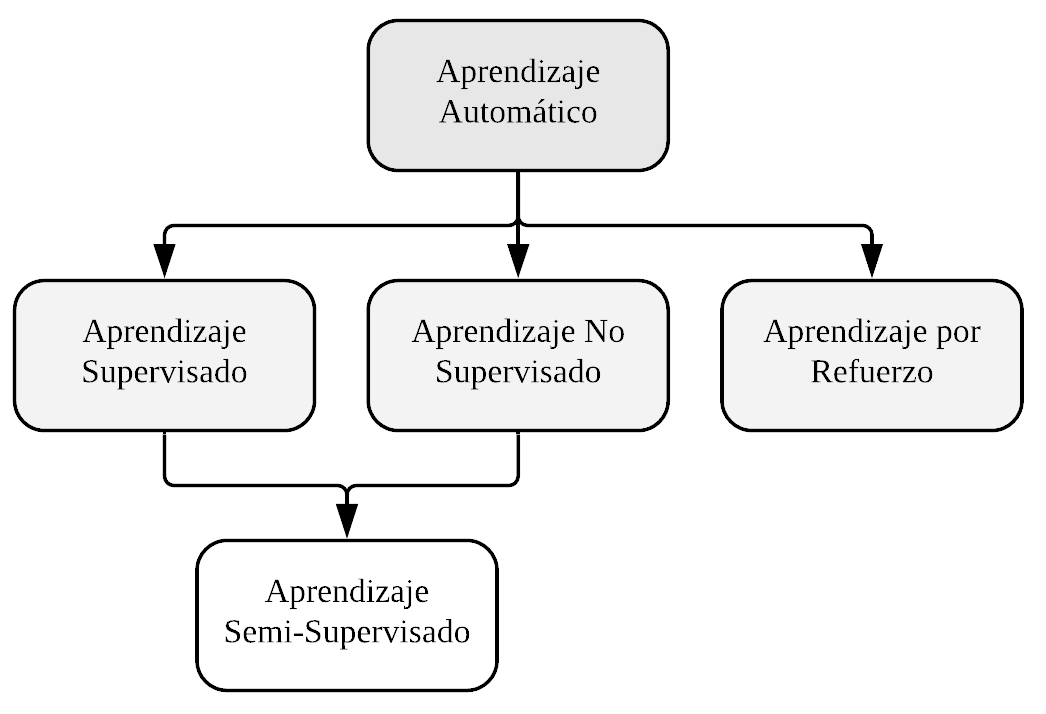
\includegraphics[width=3.5in]{figures/Figure1.png}
\caption{Clasificación de algoritmos de aprendizaje automático.}
\label{fig:1}
\end{figure}

\subsection{Aprendizaje Supervisado}

El aprendizaje supervisado es una técnica de AA que emplea datos etiquetados, llamados datos de entrenamiento, para construir un modelo predictivo, a fin de predecir la etiqueta de datos sin etiquetar.

El conjunto de datos de entrenamiento incluye datos de entrada y valores de respuesta. A partir de éste, el algoritmo de aprendizaje supervisado busca crear un modelo que pueda realizar predicciones acerca de los valores de respuesta para un nuevo conjunto de datos. Con frecuencia se utiliza un conjunto de datos de prueba para validar el modelo. Si se utilizan conjuntos de datos de entrenamiento de mayor tamaño, es posible generar modelos cuya capacidad predictiva es superior y obtener buenos resultados sobre nuevos conjuntos. \cite{Darnstadt2014}.

\subsection{Algoritmos de AA aplicados en la IR}

En esta subsección se describen los algoritmos de AA del tipo supervisado aplicados con mayor frecuencia en la IR. 

El algoritmo de aprendizaje supervisado, \textit{Máquina de Soporte Vectorial} (SVM), puede ser utilizado para tareas de clasificación o regresión binaria. Las SVM proporcionan un enfoque alternativo a la categorización de entidades y han sido ampliamente utilizadas en aplicaciones relacionadas al procesamiento de lenguaje natural, reconocimiento de voz e imagen.

Una SVM mapea los puntos de entrada a un espacio de características de una dimensión mayor (i.e. si los puntos de entrada están en \(ℜ^2\) estos son mapeados por la SVM a \(ℜ^3\)). Este algoritmo clasifica los datos al encontrar el mejor hiperplano que separe los puntos de entrada y maximice el margen \( M \) entre las clases en el espacio de características.  Los vectores de soporte son los puntos de datos más cercanos al hiperplano de separación \cite{shawe2000support}.

\textit{Naive Bayes} (NB) es un algoritmo de aprendizaje automático basado en el Teorema de Bayes con una fuerte suposición de independencia condicional entre los predictores respecto de su clase o etiqueta. En otras palabras, un clasificador NB supone que la presencia de una característica particular en una clase no está relacionada con la presencia de otra característica \cite{manning2010introduction}. Esta suposición de independencia condicional de los predictores permite al clasificador NB estimar los parámetros necesarios para una clasificación precisa mientras, usa menos datos de entrenamiento respecto a otros clasificadores. Esto lo hace particularmente efectivo para conjuntos de datos que contienen muchos predictores. 

El algoritmo \textit{K-Nearest Neighbour} (KNN) se caracteriza por ser flexible y con una mecánica fácil de entender. Este algoritmo se basa en el aprendizaje por analogía, es decir, comparando un determinado individuo de prueba o punto de interés con ejemplos de entrenamiento similares a él. Los ejemplos de entrenamiento se describen mediante n atributos. Cada ejemplo o individuo representa un punto en un espacio n-dimensional. El valor de K representa la cantidad de puntos vecinos considerados para clasificar un individuo de prueba o  punto de interés. La proximidad de los K vecinos más cercanos se define en términos de una métrica de distancia, tal como la distancia euclídea \cite{alpaydin2014introduction}.  

El algoritmo \textit{Decision Tree} (DT) es usado para resolver problemas de clasificación y regresión. Este algoritmo está basado en la lógica, donde los conjuntos de datos se modelan en estructuras jerárquicas en forma de árbol compuestas por decisiones lógicas. Cada nodo representa un atributo a evaluar, mientras que, las ramas indican las opciones de decisión sobre el atributo dado y cada hoja representa un resultado. El resultado final es una estructura de árbol donde cada nodo interno representa un condicional para el valor de un atributo y cada hoja representa la decisión para una clase en particular. En el caso de un nuevo individuo desconocido, el árbol procede a evaluar cada condicional hasta llegar al final de una de las hojas para etiquetar este nuevo caso. La complejidad del árbol se controla mediante la utilización de criterios de parada y métodos de  poda. Mientras que, las métricas utilizadas para medir la complejidad del árbol son el número de nodos, el número de hojas, la profundidad y el número de atributos utilizados \cite{rokach2005decision}. 

El algoritmo \textit{Random Forest} combina un conjunto de árboles de decisión y entrena a cada uno con un conjunto de observaciones tomadas al azar. Las predicciones finales del algoritmo se generan promediando las predicciones individuales de cada árbol.  Random Forest es un método de aprendizaje utilizado para problemas de clasificación y regresión \cite{williams2011random}. 

\subsection{Ingeniería de Requerimientos}

La IR provee el mecanismo apropiado para entender lo que desea el cliente, analizar las necesidades, evaluar la factibilidad, negociar una solución razonable, especificar la solución, validar la especificación y administrar los requerimientos a medida que se transforman en un sistema funcional \cite{thayer1997software}. Las actividades de este proceso incluyen: obtención, análisis, especificación, validación, verificación y gestión de requerimientos \cite{Pohl2010}.

Sin embargo, dada las exigencias de comunicación y colaboración entre las partes interesadas, la IR está sujeta a diversos desafíos. Especialmente, durante las actividades de educción y especificación de requerimientos, en las cuales es posible incurrir en la inserción de errores y malentendidos. Es por ello, que a menudo esta fase debe afrontar diversas dificultades, tales como especificaciones de requerimientos incompletas y ambiguas, intereses en conflicto de las partes interesadas, volatilidad en los requerimientos y restricciones de tiempo, entre otros, que influyen en la calidad y el éxito del proyecto de software. Cuando estas dificultades no son resueltas, se generan fallas, esfuerzo adicional para el equipo de desarrollo y consecuentemente, incrementan los costos del proyecto de software. 

Considerando estos retos y el surgimiento de nuevas técnicas de aprendizaje de IA, cuyo valor ha sido ampliamente reconocido en diversos dominios de aplicación, la comunidad científica ha comenzado a experimentar sobre la aplicación de diversos métodos de AA en las actividades de la IR, a fin de resolver dificultades y aspectos aún no resueltos. En los últimos años, investigadores y profesionales han explorado la utilidad del AA en aplicaciones de software para enriquecer técnicas y procedimientos tradicionales que conduzcan a contribuciones significativas en la IR. Por lo tanto, los aportes y mejoras que se puedan realizar en el área favorecerá a todo el ciclo de vida del software. Por esta razón, en esta investigación se propone brindar una visión general de la literatura acerca de cómo los investigadores han aprovechado los algoritmos de AA para automatizar y optimizar las diversas actividades involucradas en dicha área.

\section{Trabajos Relacionados}
En esta sección se describirán brevemente algunos trabajos relevantes, que buscan responder preguntas de investigación y detectar oportunidades de mejora en la IR, a fin de identificar antecedentes. La Tabla \ref{tabla1} presenta los artículos analizados y sus correspondientes preguntas de investigación.

\begin{table}[!t]
\renewcommand{\arraystretch}{1.3}
\caption{ESTUDIOS RELACIONADOS}
\label{tabla1}
\centering
\begin{tabular}{p{3cm}p{4.5cm}}
\hline
\hline Estudio & Pregunta de Investigación \\
\hline
Empirical research in requirements engineering: trends and opportunities  & RQ1.¿Cuál es el estado del arte en estudios empíricos de la IR? 

RQ2. ¿Cuál es la evidencia empírica en la literatura de IR?
\\ \cline{1-2}
Requirements Engineering Techniques: A Systematic Literature Review  & RQ1. ¿Cuáles son las técnicas utilizadas en la IR?

RQ2. ¿Cuáles son las limitaciones de las técnicas existentes utilizadas en la IR?

RQ3. ¿Cómo afectan los cambios en los requerimientos de software al análisis de requerimientos?
 \\ \cline{1-2}
A Requirements Engineering Techniques Review in Agile Software Development Methods & RQ1.¿Cuáles son los enfoques ágiles que aplican las técnicas tradicionales de la IR en los procesos de desarrollo ágil?

RQ2.¿Qué técnicas de IR se utilizan habitualmente para obtener los requerimientos de los usuarios en los procesos de desarrollo ágil?
 \\
\hline \hline                                                                                                    
\end{tabular}
\end{table}





Ambreen y otros \cite{ambreen2018empirical} presentan un mapeo sistemático en el cual definen preguntas de investigación enfocadas en la identificación de propuestas con evidencia empírica de la IR. El estudio de mapeo se basa en 270 estudios extraídos de cuatro bases de datos ACM, IEEE, SpringerLink y ScienceDirect, durante el período 1990-2012. Los resultados obtenidos reflejan que la verificación y validación de requerimientos, a pesar de su relevancia carece de evidencia empírica. Mientras que, la obtención, el análisis y la gestión de requerimientos, presentan mayor frecuencia de publicación y consecuentemente, se identifican como actividades de mayor interés. Este trabajo de investigación evidencia que las tareas relacionadas a los requerimientos no funcionales y la IR en general, son emergentes en relación a las fases que conforman el ciclo de vida de desarrollo de software. Por otro lado, el uso de ontologías y propuestas relacionadas a la detección de patrones de aplicación de las técnicas de IR en pequeñas y medianas empresas, han comenzado a ser investigadas. Finalmente, la investigación concluye que existe un interés limitado en evaluar y comparar propuestas existentes, y que la comunidad científicas se enfoca más bien, en proponer otras nuevas. Sólo el 6\% de los estudios se identificaron como trabajos empíricos. Los autores de este artículo, también detectaron que dos tercios de los artículos analizados se efectuaron en entornos empresariales controlados, sin la suficiente información  para replicar los resultados. Adicionalmente, se presenta una clasificación de las áreas emergentes de la IR en relación a las propuestas de investigación. 

Matyokurehwa y otros \cite{matyokurehwa2017requirements} examinan las técnicas de IR frecuentemente utilizadas en los proyectos de software durante el período 2000-2016. El objetivo de la investigación es hallar una relación entre las técnicas de la IR y posibles patrones de aplicación en casos concretos durante el desarrollo de un proyecto de software, además de sus limitaciones y cómo afectan a las tareas de análisis los cambios en los requerimientos. Los estudios primarios analizados presentaron cuarenta y tres (43) técnicas que abordan el análisis de los requerimientos entregados por los stakeholders, pero ninguna puede resolver de manera precisa todos los escenarios que se presentan durante el desarrollo de un proyecto. En cuanto a las limitaciones se observaron que las técnicas identificadas están circunscritas a una sola actividad de la IR. Por último, los autores de este trabajo identificaron que los cambios no previstos pueden generar potenciales problemas con el presupuesto y la estimación del tiempo de entrega de los hitos del proyecto. Esta investigación señala como potencial laguna de investigación, el desarrollo de técnicas que aborden las actividades de la IR. Considerando que es necesario idear técnicas que sean fáciles de monitorear y adoptar en los proyectos de desarrollo de software.

Zamudio y otros \cite{zamudio2017requirements} presentan una revisión que aborda temas relacionados a las aplicaciones de las técnicas tradicionales de la IR en las metodologías ágiles de desarrollo de software. En particular, los autores analizaron las siguientes metodologías ágiles: SCRUM, Dynamic Systems Development Method (DSDM), Adaptive Software Development (ASD) y Crystal Family. Los resultados obtenidos permiten determinar que las  técnicas tradicionales de la IR son aplicadas en las metodologías ágiles sin identificar un patrón acerca de su uso. En el caso de eXtreme Programming (XP), Scrum y Crystal se identificaron las siguientes técnicas para la tarea de educción de requisitos: entrevistas, lluvia de ideas, priorización, modelado de requerimientos, construcción de escenarios y casos de usos. Mientras que para el análisis de los requerimientos frecuentemente se adoptan, los diagramas de lenguaje unificado de  modelado (UML). Los autores concluyen su trabajo sosteniendo que los métodos ágiles no poseen técnicas diferentes a las usadas en las metodologías tradicionales para la extracción de requerimientos, aún más éstas poseen flujos de trabajos donde se aplican las técnicas tradicionales de la IR continuamente, a medida que los requerimientos van mutando.

Luego del análisis de estas propuestas es posible concluir que la IR es reconocida como una subdisciplina de la Ingeniería de Software emergente y con lagunas de investigación. El objetivo del análisis de los trabajos mencionados anteriormente, es obtener antecedentes y detectar puntos de interés en común que permitan argumentar y justificar el desarrollo de esta investigación. A pesar que las investigaciones analizadas abordan alcances y preguntas de investigación distintas a las definidas en este artículo, todas coinciden en la necesidad de enriquecer y mejorar dicha área, la cual es esencial para el éxito de un proyecto de software. Estamos convencidos que la IR puede hallar oportunidades de mejora y beneficiarse de la aplicación de nuevas tecnologías y métodos, tales como el AA y es este aspecto el que analizaremos en esta investigación.  


\section{Metodología}

El método utilizado para desarrollar este mapeo sistemático de la literatura se basa en los lineamientos establecidos en las contribuciones de Petersen y otros \cite{petersen2008systematic}, una propuesta ampliamente aceptada por la comunidad científica para realizar estudios de mapeo en el área de la Ingeniería de Software. El proceso de investigación consta de cinco etapas principales: (a) definición de las preguntas de investigación, (b) búsqueda e identificación de estudios primarios mediante cadenas de búsqueda en bibliotecas académicas digitales, (c) selección de los estudios mediante criterios de inclusión y exclusión, (d) revisión de estudios seleccionados a través de la lectura comprensiva de resúmenes, búsqueda de palabras clave y conceptos que reflejen el contexto de investigación, y por último, e) extracción y análisis de datos. La Fig. \ref{fig:2} sintetiza el método aplicado en esta investigación.

Las subsecciones posteriores, describen los elementos de entrada y salidas obtenidos como resultado de la metodología aplicada.

\subsection{Preguntas de Investigación}

Esta investigación identifica propuestas que aplican técnicas de AA del tipo supervisado para resolver desafíos que surgen durante las actividades de la IR. A fin de definir el alcance de este artículo se formularon tres preguntas de investigación. La Tabla \ref{tabla12} presenta las preguntas y los criterios que motivan su formulación. 

La primera pregunta tiene por objetivo identificar las tareas y  actividades de la IR que han sido abordadas, mediante el uso de las técnicas de AA  en diversas contribuciones académicas halladas en la literatura. La finalidad es descubrir tendencias respecto a la aplicación de estas técnicas  y determinar las actividades que han resultado más beneficiadas, a partir de estos aportes y propuestas. El propósito de la segunda pregunta es determinar posibles correspondencias de uso entre los algoritmos de AA aplicados en las diversas propuestas y las actividades y/o desafíos de la IR. Por último, la tercera pregunta pretende identificar y difundir los conjuntos de datos disponibles en la web y la literatura, a fin proveer a los profesionales de este campo de estudio, recursos que faciliten la prueba y validación de los modelos AA. 

\begin{table}[!t]
\renewcommand{\arraystretch}{1.3}
\caption{PREGUNTAS DE INVESTIGACIÓN}
\label{tabla12}
\centering
\begin{tabular}{p{3cm}p{4.5cm}}
\hline
\hline
Pregunta de Investigación & Motivación \\
\hline
Q1. ¿Cuáles son las actividades de la IR respaldadas por el 
aprendizaje supervisado?  & M1. Identificar propuestas que 
utilizan el aprendizaje supervisado para abordar las 
actividades de la IR.\\ \cline{1-2}
Q2. ¿Cuáles son los algoritmos de aprendizaje supervisado utilizados para resolver dificultades en las actividades de la IR? & M2. Detectar los principales algoritmos de aprendizaje supervisado aplicados para resolver dificultades y desafíos presentes en la IR. \\ \cline{1-2}
Q3. ¿Cuáles son las principales fuentes de datos utilizadas para ejecutar los algoritmos de aprendizaje supervisado? & M3. Identificar repositorios y fuentes de datos utilizados como entrada para la ejecución de los algoritmos de aprendizaje supervisado. \\
\hline \hline                                                                                                    
\end{tabular}
\end{table}



\subsection{Estrategia de Búsqueda}

Los estudios se identificaron consultando cuatro bibliotecas en línea: (i) IEEEXplore; (ii) ScienceDirect; (iii) SpringerLink y (iv) Scopus. Estas bibliotecas fueron seleccionadas porque son consideradas fuentes importantes de estudios en el área Informática en general, y de Ingeniería de Software en particular, poseen repositorios de conferencias y revistas relevantes. Asimismo, sus motores de búsqueda admiten la posibilidad de realizar búsquedas avanzadas basadas en diferentes criterios y formatos de cadena.

Los términos utilizados para construir la consulta de búsqueda fueron acordados entre los autores, teniendo en cuenta las directrices propuestas por Petersen y otros \cite{petersen2008systematic}. Estos se mencionan a continuación: (1) Identificar los términos principales en las preguntas de investigación; (2) Extraer palabras clave de documentos relevantes a la temática; (3) Identificación de términos de búsqueda en títulos, resúmenes y palabras clave relevantes; (4) Identificar sinónimos y abreviaturas alternativas; (5) Construir cadenas de búsqueda, concatenando las palabras identificadas mediante operadores booleanos "AND" para enlazar los términos principales y "OR" para incorporar sinónimos alternativos. La cadena de búsqueda genérica resultante se muestra en la Fig. \ref{fig:3}.

La misma fue adaptada a la sintaxis de los motores de búsqueda de cada repositorio. Si bien, este trabajo aborda el análisis de las investigaciones que aplican aprendizaje supervisado, en las simulaciones de búsqueda realizadas se observó la presencia de estudios vinculados a la temática que utilizaron como palabra clave el término aprendizaje automático sin especificar el tipo de enfoque de aprendizaje aplicado (supervisado, no supervisado, semi-supervisado, por refuerzo).

\begin{figure}[!t]
\centering
\includegraphics[width=3.5in]{figures/figure2_Guada.png}
\caption{Metodología de investigación \cite{petersen2008systematic}.}
\label{fig:2}
\end{figure}


\begin{figure}[!t]
\centering
\includegraphics[width=3.5in]{figures/figure3_Guada.png}
\caption{Cadena de búsqueda genérica.}
\label{fig:3}
\end{figure}

Es por ello, que se añadió este término a la cadena de búsqueda.

Con la intención de impulsar a los investigadores a trabajar en propuestas innovadoras y alentar a la comunidad en general a trabajar en nuevas tecnologías de AA, en el año 2002 fue liberada la librería Torch. Una librería de AA bajo licencia de código abierto BSD, distribución de software Berkeley, que 
incluye los algoritmos y modelos más populares, tales como máquina de soporte vectorial (SVM), modelos gaussianos mixtos, clasificadores bayesianos, K-vecinos más cercanos (KNN), redes neuronales artificiales (ANN), entre otros \cite{collobert2002torch}.

La difusión de este hecho y el creciente interés en indagar más aún sobre la utilidad de las técnicas de AA impulsó su aplicación en diversos dominios. Consecuentemente, por esta razón, la búsqueda de estudios en este trabajo se acotó al período que parte desde el citado hito hasta el año 2018, planteando como desafío descubrir oportunidades de investigación y lagunas en el campo del aprendizaje supervisado aplicado a la IR.
\subsection{Criterios de Inclusión y Exclusión}

Esta investigación se centra en el análisis de propuestas cuyo foco de investigación es la aplicación de técnicas de aprendizaje automático supervisado en la IR. Fueron incluidas publicaciones redactadas en idioma inglés, debido al bajo nivel de difusión de publicaciones y artículos redactados en otros idiomas en revistas relevantes de Ingeniería de Software. 

Los términos incluidos en la cadena de búsqueda deben aparecer al menos en el título, resumen o palabras clave, lo que contribuye a identificar los artículos que se centran en el tema de análisis. Se incluyeron artículos revisados por pares publicados en el período 2002-2018, considerando como un hito relevante en el campo del AA, la liberación de la librería Torch.

\begin{table}[!t]
\renewcommand{\arraystretch}{1.3}
\caption{CRITERIOS DE INCLUSIÓN Y EXCLUSIÓN}
\label{tabla2}
\centering
\begin{tabular}{p{3.5cm}p{4cm}}
\hline
\hline
Criterios de Inclusión & Criterios de Exclusión \\
\hline
CI1. Trabajos de investigación con propuestas concretas en la aplicación de técnicas de aprendizaje automático supervisado en las actividades de IR  & CE1. Trabajos de investigación cuya aplicación de técnicas de aprendizaje automático supervisado,
pertenezcan a un contexto distinto al de IR.\\ \cline{1-2}
CI2. Estudios publicados en librerías digitales entre los años 2002 y 2018 & CE2. Propuestas e investigaciones
cuya profundidad temporal excedan del intervalo de tiempo especificado para la elaboración del mapeo sistemático. \\ \cline{1-2}
CI3. La cadena de búsqueda debe aparecer en el título, resumen o palabras clave del estudio & CE3. Estudios que no contengan en título, resumen o palabras clave, los términos utilizados en la cadena de búsqueda. \\ \cline{1-2}
CI4. Estudios publicados en idioma inglés. & CE4. Trabajos de investigación no redactados en idioma inglés. \\
\hline \hline                                                                                                    
\end{tabular}
\end{table}

\begin{figure}[!t]
\centering
\includegraphics[width=3.5in]{figures/figure4_Guada.png}
\caption{Número de estudios identificados por repositorio acad\'emico.}
\label{fig:4}
\end{figure}

Fueron excluidos los estudios no revisados por pares, duplicados, no redactados en inglés, documentos redundantes de la misma autoría, documentos del tipo tesis, position papers, panel de discusiones y, aquellos que no incluían técnicas de aprendizaje automático supervisado para apoyar las actividades de IR. La Tabla \ref{tabla2} resume los criterios de inclusión y exclusión considerados para seleccionar los estudios candidatos al análisis.

\subsection{Extracción de Datos}

La cadena de búsqueda se aplicó en los repositorios seleccionados, sobre títulos, resúmenes y palabras clave. Fueron identificados doscientos sesenta y nueve (269) documentos como resultado de la ejecución. La biblioteca IEEEXplore devolvió veintiséis (26) artículos; Scopus sesenta y dos (62); ScienceDirect identificó sólo cinco (5) documentos; y finalmente, SpringerLink fue la biblioteca que retornó una mayor cantidad, identificando ciento setenta y seis (176) artículos. La Fig. \ref{fig:4} sintetiza la cantidad de estudios recuperados por repositorio académico y los artículos seleccionados.

Los artículos recuperados de los repositorios académicos fueron organizados en un formulario de extracción de datos, por título, año de publicación y revista o conferencia. Cada uno de estos artículos fueron analizados en busca de aquellos que cumplían los criterios de inclusión, mientras que los que no cumplían con éstos fueron excluidos. 

Como resultado del proceso de filtrado, fueron seleccionados treinta y uno (31) documentos que detallan explícitamente la implementación de técnicas de aprendizaje supervisado en el área de la IR. La estrategia de "bola de nieve hacia atrás" \cite{wohlin2014guidelines} se aplicó posteriormente para detectar estudios asociados con la temática de investigación. Esta estrategia consiste en revisar las referencias bibliográficas citadas en los estudios identificados como relevantes para reconocer artículos relacionados a la temática de investigación. Como resultado de este proceso, se añadieron dos (2) estudios. El número total de estudios candidatos para el proceso de revisión y análisis fue treinta y tres (33).

\subsection{Síntesis de Datos }

Esta investigación analiza treinta y tres (33) estudios, resultantes del proceso de selección. A continuación, se detallan los resultados obtenidos y luego, se responden las preguntas de investigación.

La distribución de los estudios publicados en función del tiempo permite visualizar las tendencias respecto al empleo de técnicas de aprendizaje supervisado en el área de la IR. La Fig. \ref{fig:5} muestra la distribución de los artículos seleccionados por año de publicación.

\begin{figure}[!t]
\centering
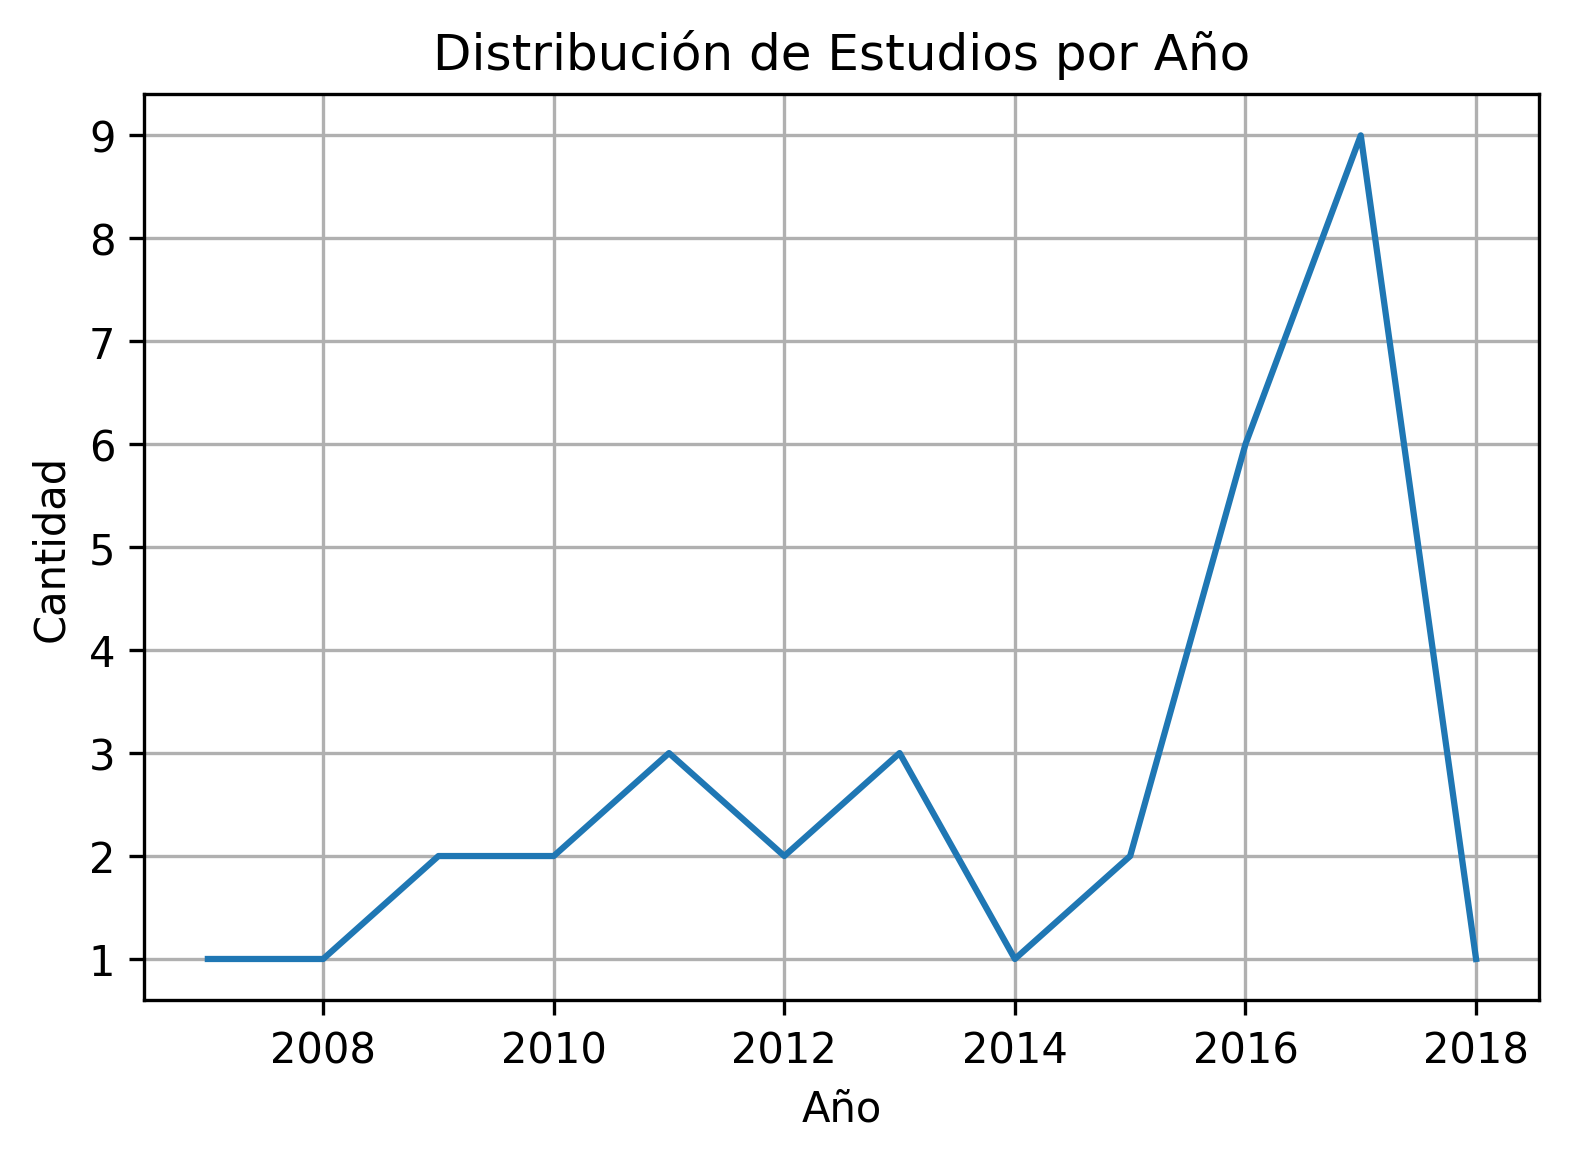
\includegraphics[width=3.5in]{figures/Figure5_Guada.png}
\caption{Distribuci\'on de estudios seleccionados por año de publicaci\'on.}
\label{fig:5}
\end{figure}


\begin{figure}[!t]
\centering
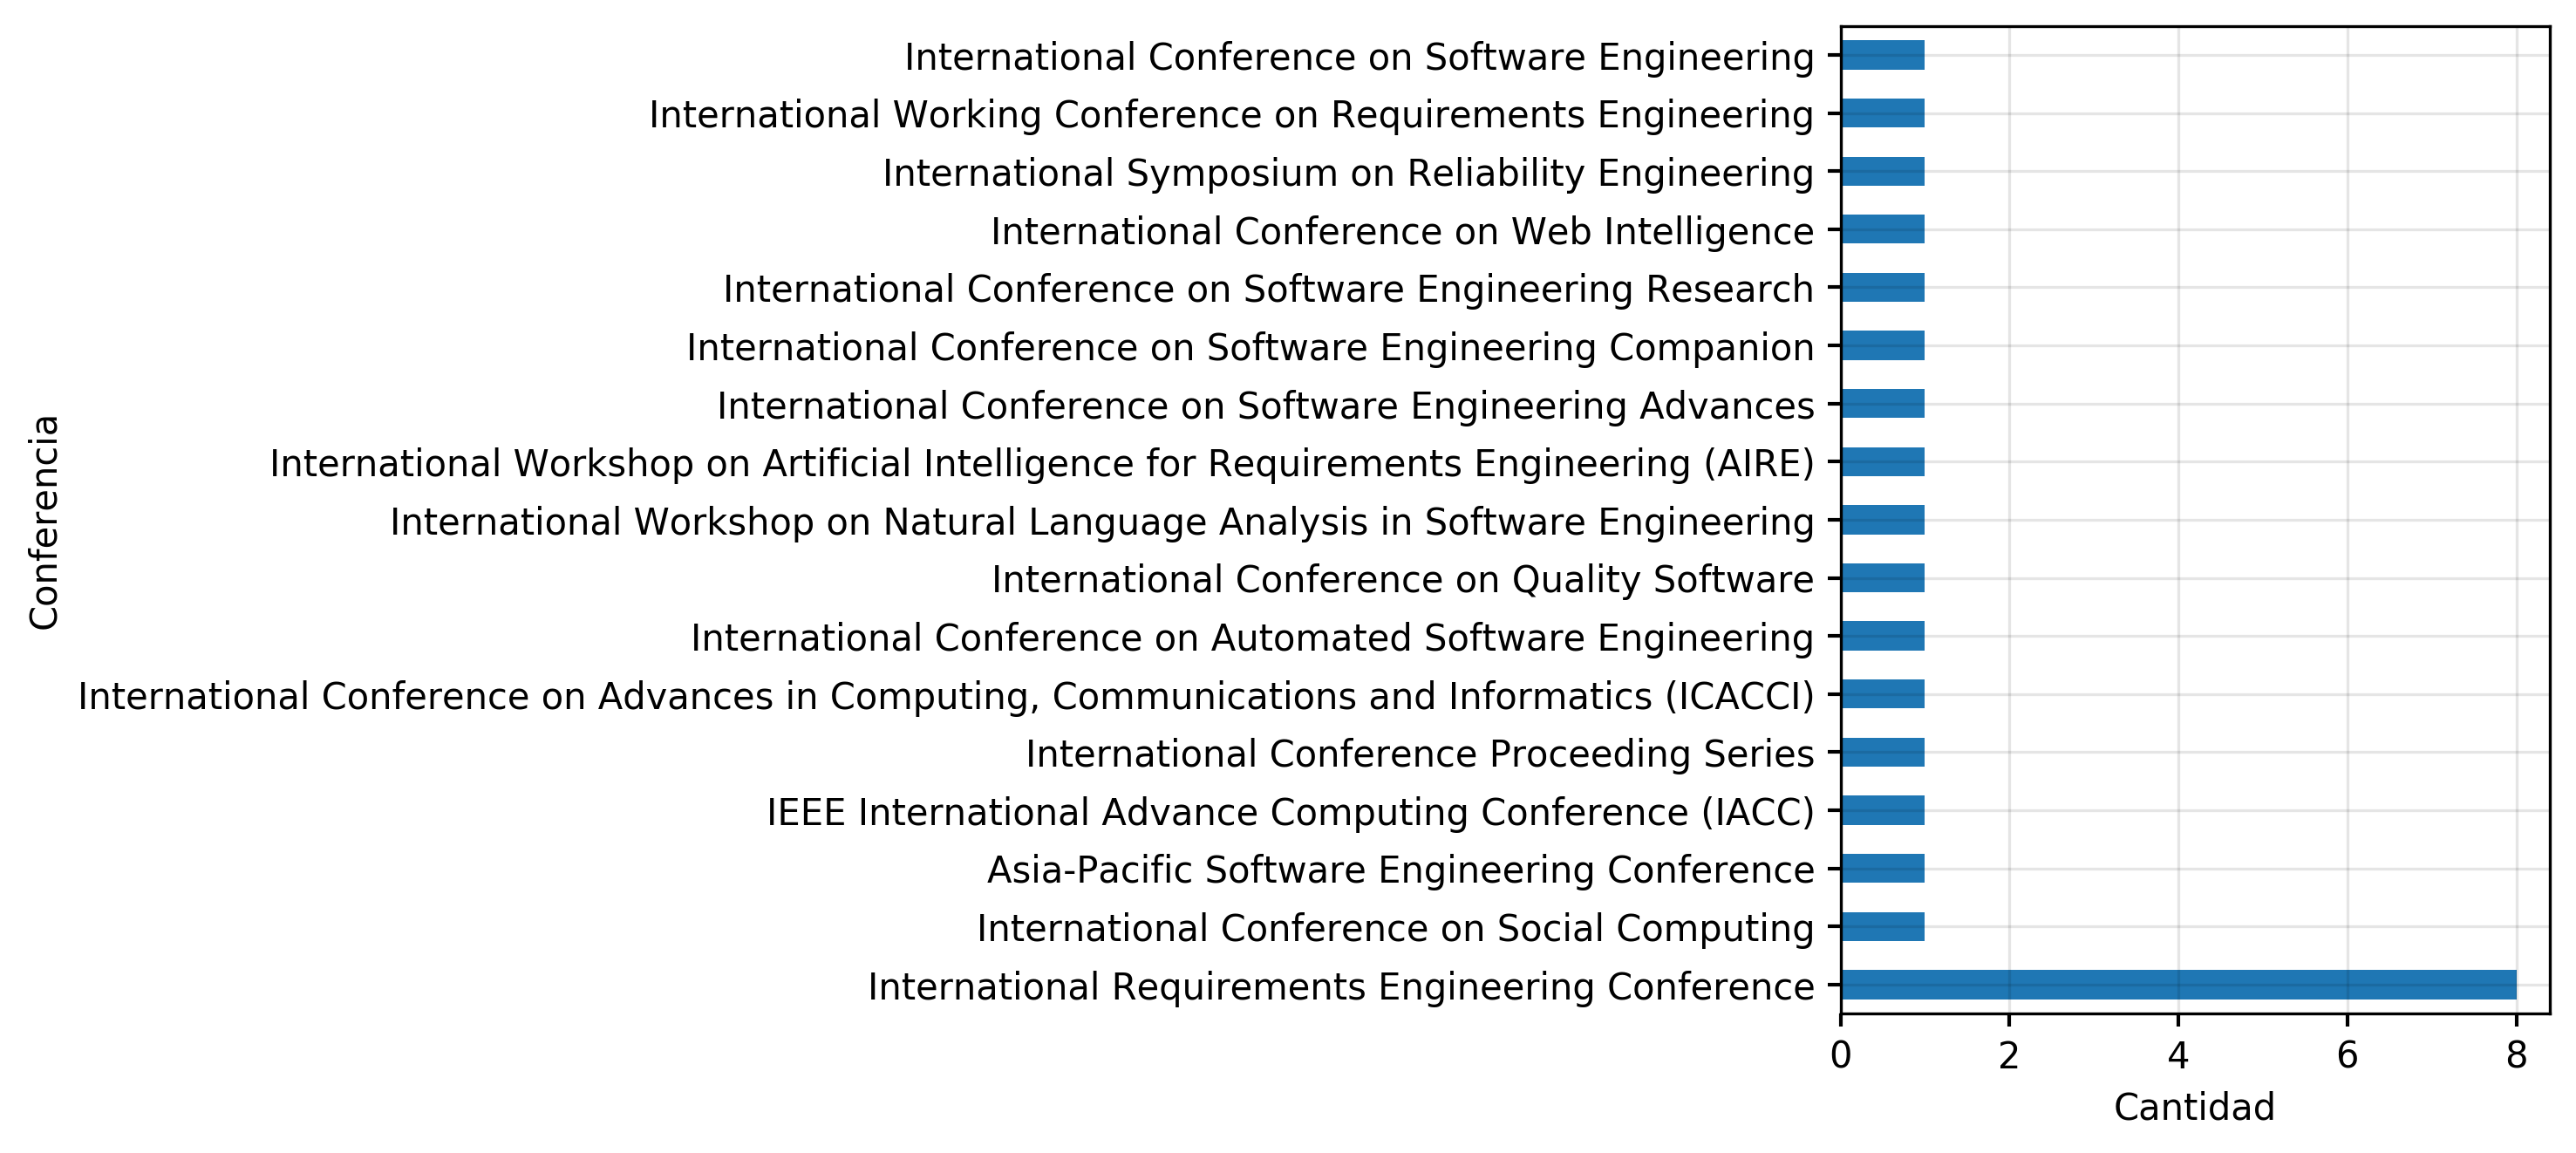
\includegraphics[width=3.5in]{figures/Figure6_Guada.png}
\caption{Distribuci\'on de estudios publicados en conferencias cient\'ificas.}
\label{fig:6}
\end{figure}

\begin{figure}[!t]
\centering
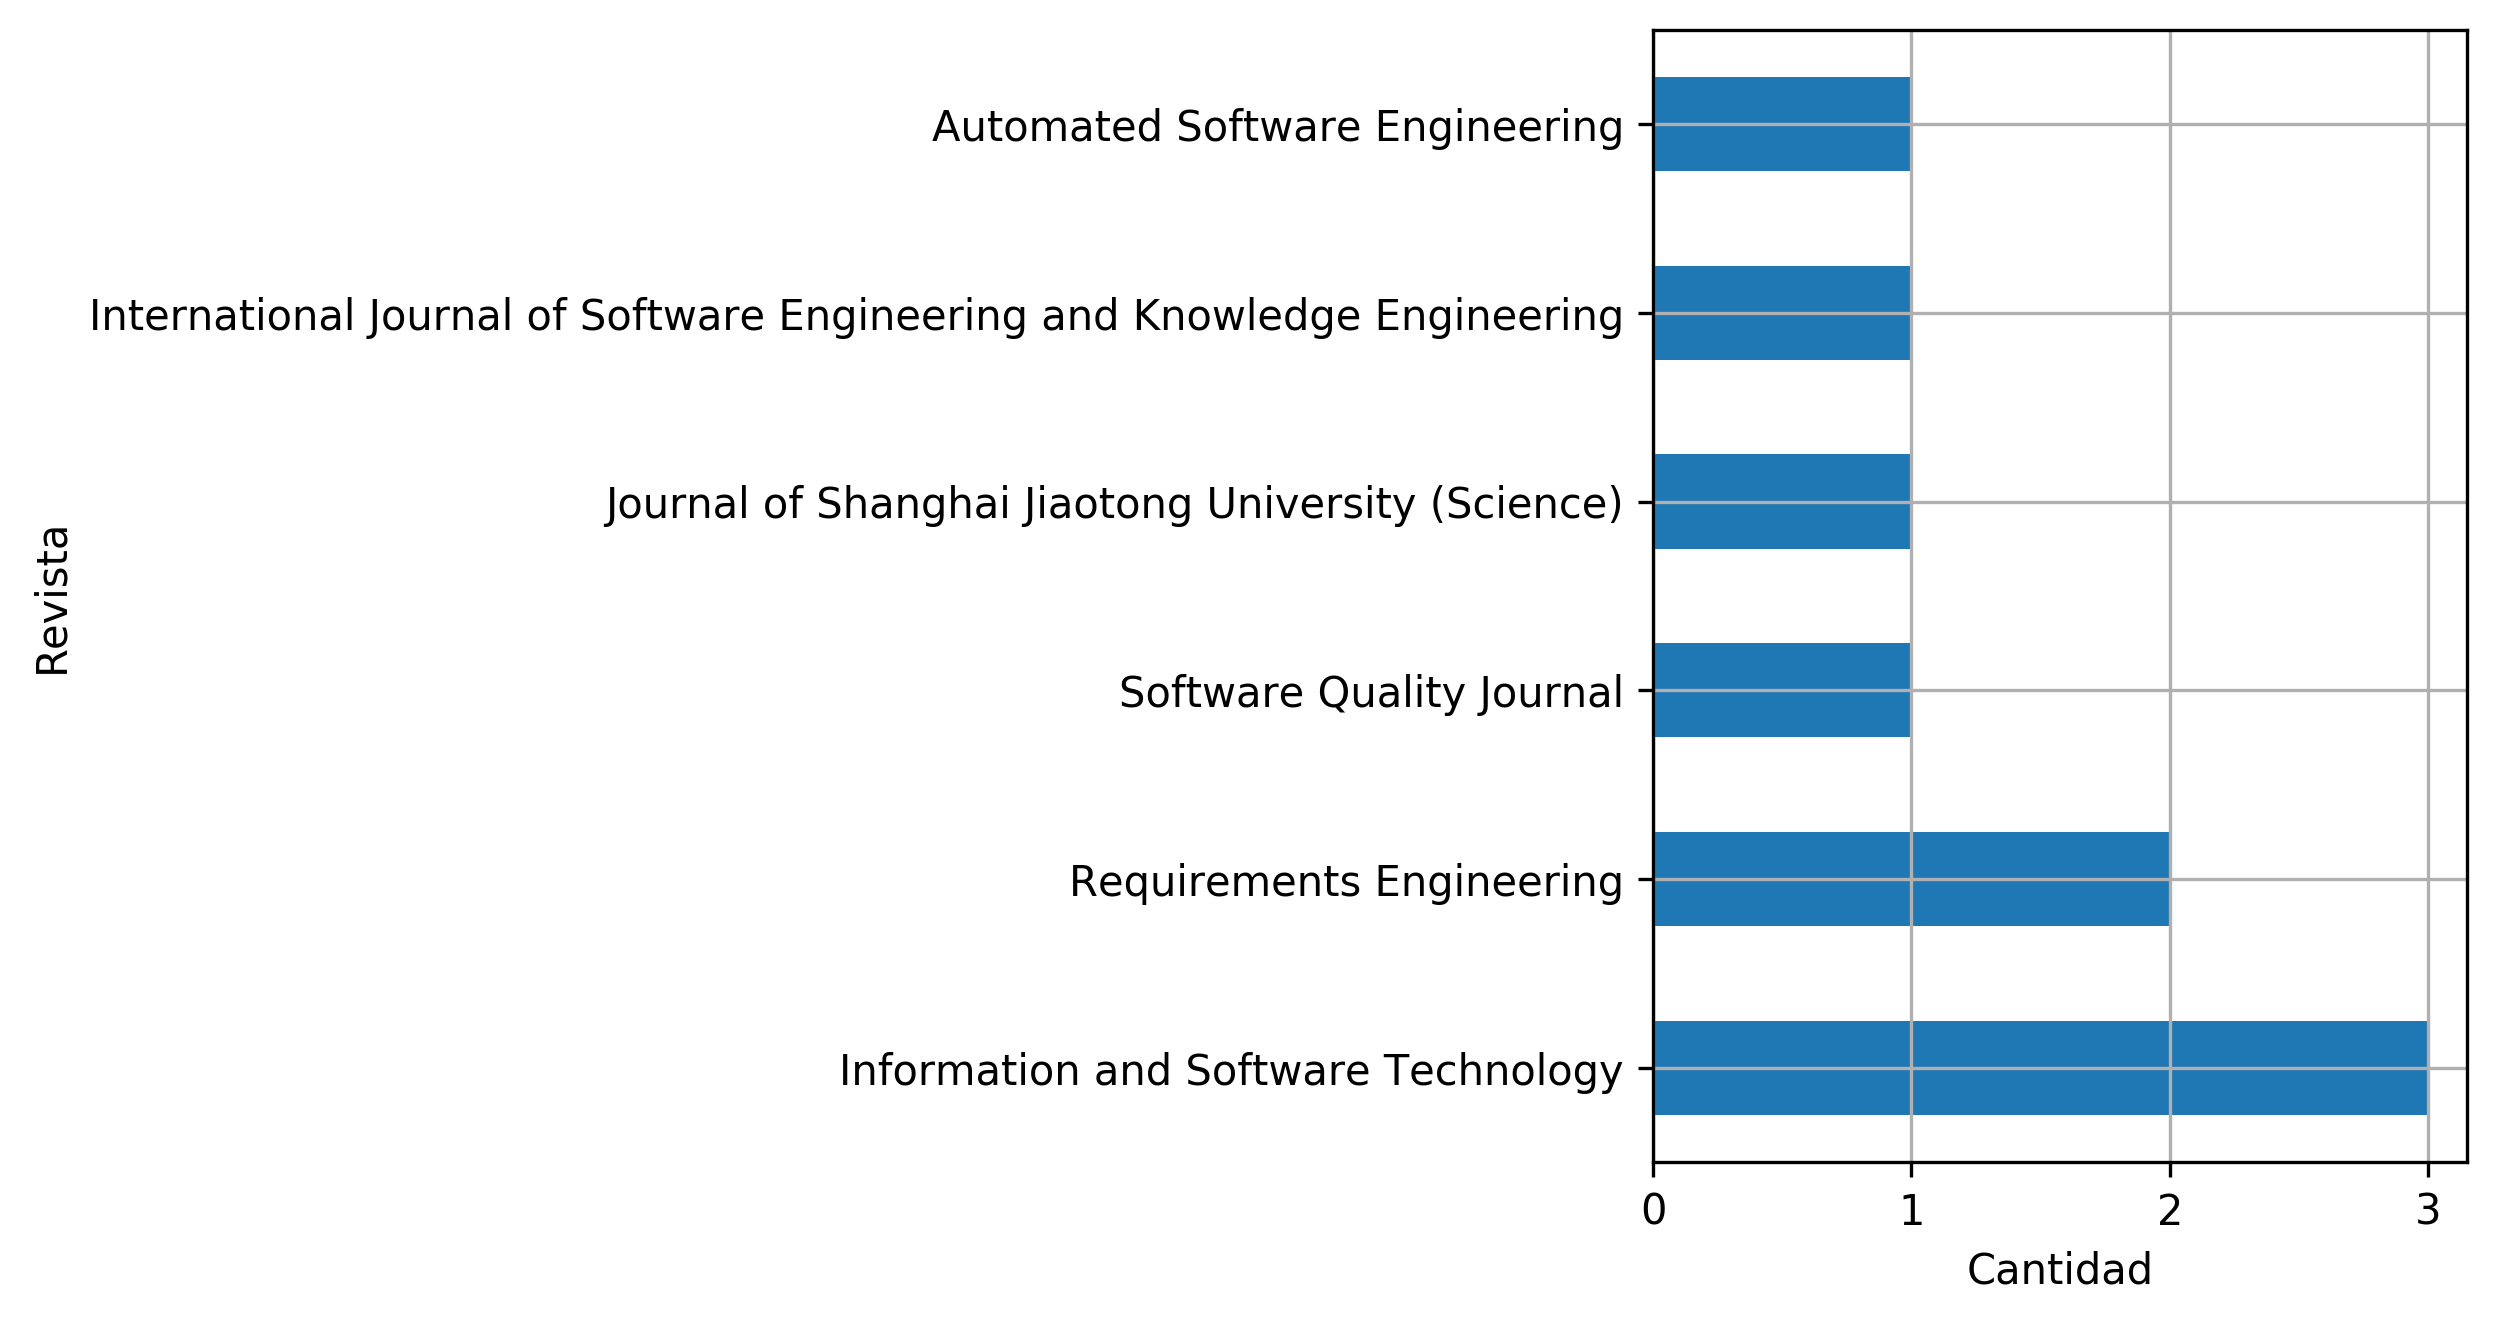
\includegraphics[width=3.5in]{figures/Figure7_Guada.png}
\caption{Distribuci\'on de estudios seleccionados por año de publicaci\'on en revistas científicas.}
\label{fig:7}
\end{figure}

La Fig. \ref{fig:5} muestra un aumento significativo del 67\% respecto a propuestas de investigación que utilizan métodos de aprendizaje supervisado para dar soporte a las diversas tareas de la IR durante el período (2016-2018). En consecuencia, es notable el posicionamiento de las tecnologías de AA como tema de interés en los últimos dos años. Probablemente, esto se deba a los importantes avances respecto al incremento de la capacidad de procesamiento en los ordenadores y el surgimiento de nuevas técnicas que otorgan mayor poder de aprendizaje. Otro aspecto relevante, es el reconocimiento de la comunidad científica respecto al valor del AA para automatizar tareas y resolver dificultades en diversos dominios, lo que sin dudas ha motivado a los profesionales de la IR a investigar sobre su uso en dicha área. Con la finalidad de ampliar las capacidades y recursos de los desarrolladores para brindar soluciones inteligentes a los desafíos presentes en la IR. 

Como se mencionó anteriormente, un mapeo sistemático tiene como objetivo identificar las revistas y conferencias científicas utilizadas frecuentemente por los investigadores para difundir sus trabajos de investigación. Es por ello, que en la Fig. \ref{fig:6} se identifican las conferencias más populares y su frecuencia de publicación, a fin de reconocer los potenciales espacios para presentar futuras propuestas. 

En esta investigación se identificaron veinticuatro (24) estudios publicados en conferencias internacionales. La conferencia que presenta mayor frecuencia de publicación, ocho (8) estudios, es la “International Requirements Engineering Conference”. Esta conferencia está clasificada con la categoría A en el ranking de Excelencia en Investigación en Australia (ERA) y con la categoría A1 en el ranking de Qualis del Ministerio de Educación de Brasil. Probablemente su elevada categoría, sea una de las razones que justifica la frecuencia de publicación en dicha conferencia. 

En cuanto a publicaciones en revistas científicas fueron identificados nueve (9) artículos. La Fig. \ref{fig:7} señala las revistas más populares y su frecuencia de publicación. De acuerdo a los resultados obtenidos se observa que la revista “Information and Software Technology” posee tres (3) artículos publicados, mientras que, "Requirements Engineering" posee dos (2) artículos publicados en los últimos quince años. Ambas revistas forman parte del cuartil (Q2), escala que ofrece scimagojr\footnote{https://www.scimagojr.com/}, para clasificar revistas relevantes. 

A continuación, se responden las preguntas de investigación definidas.

\emph{\textbf{Q1. ¿Cuáles son las actividades de la IR respaldadas por las técnicas de aprendizaje supervisado?}}

Los artículos identificados demuestran que el aprendizaje supervisado, es utilizado en la actualidad por ingenieros e investigadores para obtener nuevas perspectivas y soluciones a problemas que anteriormente se encontraban fuera de su alcance, aprovechando la infraestructura de hardware y una mayor disponibilidad de los datos. El Anexo A presenta un resumen de los estudios seleccionados.

En esta investigación se identificaron métodos y propuestas que apoyan las tareas de obtención y especificación de requerimientos. La obtención de requerimientos es la tarea que determina, a través de la comunicación con los clientes y usuarios, las necesidades y restricciones del producto software a desarrollar.
 
Los requerimientos se obtienen a través de entrevistas, inspecciones, cuestionarios, entre otras técnicas, a los stakeholders. Es una tarea compleja, porque requiere una comunicación eficiente, a los fines de especificar posteriormente lo recopilado en un documento formal de requerimientos. Es por ello, que los requerimientos deben concebirse sin ambigüedades para definir de manera correcta lo que los stakeholders esperan que haga el sistema.

En esta revisión, se identificaron cinco (5) propuestas que abordan los desafíos relacionados con la detección de incertidumbre \cite{yang2012speculative}, \cite{Knauss201685} y ambigüedad \cite{yang2010extending}, \cite{Yang2011}, \cite{Ott2013} en documentos de requerimientos y artefactos escritos en lenguaje natural. Estas propuestas tienen por objeto ayudar a los analistas e ingenieros a identificar los requerimientos propensos a generar malentendidos entre las partes interesadas.


Por otro lado, determinar la coherencia respecto a un documento de requerimientos también es una tarea abordada mediante las técnicas de aprendizaje supervisado \cite{nikora2009automated}. Sólo se identificó un (1) estudio en el área. Esta propuesta utiliza técnicas de procesamiento de lenguaje natural y aprendizaje supervisado para identificar tipos específicos de requerimientos dentro de un conjunto de especificaciones y generar subconjuntos. Esto facilita el análisis de cada subconjunto respecto a aspectos tales como consistencia, integridad y ambigüedad en relación a otros requerimientos. La agrupación de requerimientos en muestras de menor tamaño minimiza la probabilidad de errores durante su análisis.

Otras investigaciones abordan la clasificación automática de los requerimientos escritos en lenguaje natural en requerimientos funcionales (RF) y las diversas subcategorías de los requerimientos no funcionales (RNF). Esto se debe particularmente, al hecho de que los stakeholders, al igual que los ingenieros de requerimientos, usan diversas terminologías y estructuras de oraciones para describir el mismo tipo de requerimiento. Dados estos problemas, es imperativo desarrollar nuevas técnicas y herramientas que puedan respaldar la clasificación de requerimientos. En este trabajo se identificaron ocho (8) propuestas que apuestan a resolver este desafío mediante la aplicación de técnicas de aprendizaje supervisado \cite{li2017identifying,Jindal20162027,kurtanovic2017automatically,dekhtyar2017re,abad2017works,Slankas2013,Slankas2013a}.

Merten y otros \cite{Merten2016} en su propuesta aplican técnicas de aprendizaje supervisado y procesamiento de textos para detectar y clasificar solicitudes de funcionalidades de software presentes en los sistemas de seguimiento y soporte a problemas.

Los documentos de requerimientos, además de contener especificaciones, poseen contenido auxiliar, tales como, resúmenes, explicaciones, referencias a otros documentos, entre otros. Se detectó un (1) estudio que aborda la categorización del contenido de las especificaciones, clasificándolo por requerimiento o información \cite{winkler2016automatic}, a fines de simplificar el trabajo de ingenieros y analistas de requerimientos.

Otras investigaciones tienen como foco de estudio los enlaces de trazabilidad, fundamentales para el mantenimiento del producto software porque establecen vínculos entre los artefactos de software relacionados, por ejemplo, código fuente, documentación, especificaciones de requerimientos, entre otros, dentro de un sistema. Esto implica que un requerimiento sea trazable desde su definición y durante todo el desarrollo del software, lo cual garantiza una adecuada gestión de cambios y evaluación de impacto en el resto del sistema. La identificación y clasificación de la trazabilidad entre los requerimientos es abordada en seis (6) propuestas \cite{Li201725}, \cite{Cleland-Huang2010,gokyer2008non,Mills2017,Sardinha2013,AtasM.2018}.

La identificación de reglas de negocio es una tarea importante del proceso de la IR. Sin embargo, resulta desafiante ya que estas reglas a menudo, no se establecen explícitamente en los documentos de requerimientos. En caso de que las reglas de negocio sean explícitas, pueden no ser de naturaleza atómica, o pueden ser vagas. Los hallazgos en esta investigación demuestran que el aprendizaje supervisado ha sido empleado para detectar reglas de negocio sobre las especificaciones de requerimientos\cite{sharma2014automated}. Se identificó sólo un (1) estudio que propone una solución a dicho desafío.

Uno de los factores más importantes y desafiantes en el desarrollo de un proyecto de software, es la obtención de requerimientos de calidad. Los requerimientos erróneos no detectados en fases tempranas pueden provocar costos adicionales, insatisfacción de las partes interesadas y retrasos en la entrega del producto software, consecuentemente, esto podría generar la cancelación del proyecto. Por estas razones, la investigación sobre dicha temática resulta clave. En este trabajo se identificaron tres (3) estudios que abordan la clasificación y evaluación de la calidad de requerimientos \cite{Parra2015180,Hayes2015,Hussain2007}. 

Algunas investigaciones utilizan el aprendizaje supervisado para hacer predicciones respecto a la necesidad de revisión en los documentos de requerimientos \cite{del2017stability} con el objetivo de ayudar a los analistas e ingenieros a determinar si una especificación de requerimientos es lo suficientemente estable o necesita revisión adicional. Además, estas técnicas también son utilizadas para predecir el rendimiento operativo del sistema mediante el análisis de la calidad de los requerimientos \cite{dargan2016systems}. Otros aplican el aprendizaje supervisado para predecir fallas en las funcionalidades solicitadas por los stakeholders en los sistemas de gestión de solicitudes de funciones en línea \cite{fitzgerald2012early}, predicción de clases en el código propensas al cambio \cite{malhotra2017exploratory}, predicción de riesgos en los requerimientos, con la intención de obtener predictores que indiquen la necesidad de utilizar técnicas para la gestión de riesgos y así mitigar su impacto \cite{del2011requirement}. Se identificaron cinco (5) propuestas que resuelven desafíos de la IR mediante la generación de modelos predictivos. 

Por otro lado, se detectó un enfoque que emplea el aprendizaje supervisado para cuantificar el impacto de los RNF en la estimación del esfuerzo de desarrollo de un proyecto de software \cite{Abdukalykov2011158}. También, se identificó una propuesta que aborda el análisis de requerimientos para extraer automáticamente información semántica \cite{Wang2016}. 

A partir del análisis de los estudios seleccionados, es notable el amplio abanico de aplicaciones de modelos de aprendizaje supervisado en el campo de la IR. Especialmente, se destacan las propuestas destinadas a resolver problemas lingüísticos presentes en los documentos de requerimientos y artefactos escritos en lenguaje natural. Por otro lado, también se distinguen las investigaciones enfocadas en la clasificación del contenido de los documentos de requerimientos.


\begin{table}[!t]
\renewcommand{\arraystretch}{1.3}
\caption{ARTÍCULOS POR CATEGORÍA Y ACTIVIDADES DE LA IR}
\label{tabla3}
\centering
\begin{tabular}{p{2.8cm}p{1.7cm}p{3cm}}
\hline
\hline
Categoría & ID Articulo & Actividades de la IR \\
\hline
Análisis de Requerimientos & \cite{Wang2016} & Análisis de Requerimientos \\ \cline{1-3}
Reglas de Negocio & \cite{sharma2014automated} & Especificación de Requerimientos \\ \cline{1-3}
Clasificación de Contenido & \cite{li2017identifying,Jindal20162027,kurtanovic2017automatically,dekhtyar2017re,abad2017works,Slankas2013,Slankas2013a,Merten2016,winkler2016automatic} & Análisis de Requerimientos \\ \cline{1-3}
Predicción de Fallas & \cite{del2017stability,dargan2016systems,fitzgerald2012early,malhotra2017exploratory,del2011requirement} & Validación y Verificación \\ \cline{1-3}
Estimación de Esfuerzo & \cite{Abdukalykov2011158} & Validación y Verificación\\ \cline{1-3}
Problemas lingüísticos en documentos de requerimientos y
artefactos escritos en lenguaje natural (PDNL) &\cite{yang2010extending,yang2012speculative,Knauss201685,Yang2011,Ott2013,nikora2009automated} & Validación y Verificación \\ \cline{1-3}
Trazabilidad &\cite{Li201725,Cleland-Huang2010,gokyer2008non,Mills2017,Sardinha2013,AtasM.2018} & Especificación de Requerimientos  \\ \cline{1-3}
Calidad & \cite{Parra2015180,Hayes2015,Hussain2007} & Especificación de Requerimientos \\
\hline \hline                                                                                                    
\end{tabular}
\end{table}

\begin{figure}[!t]
\centering
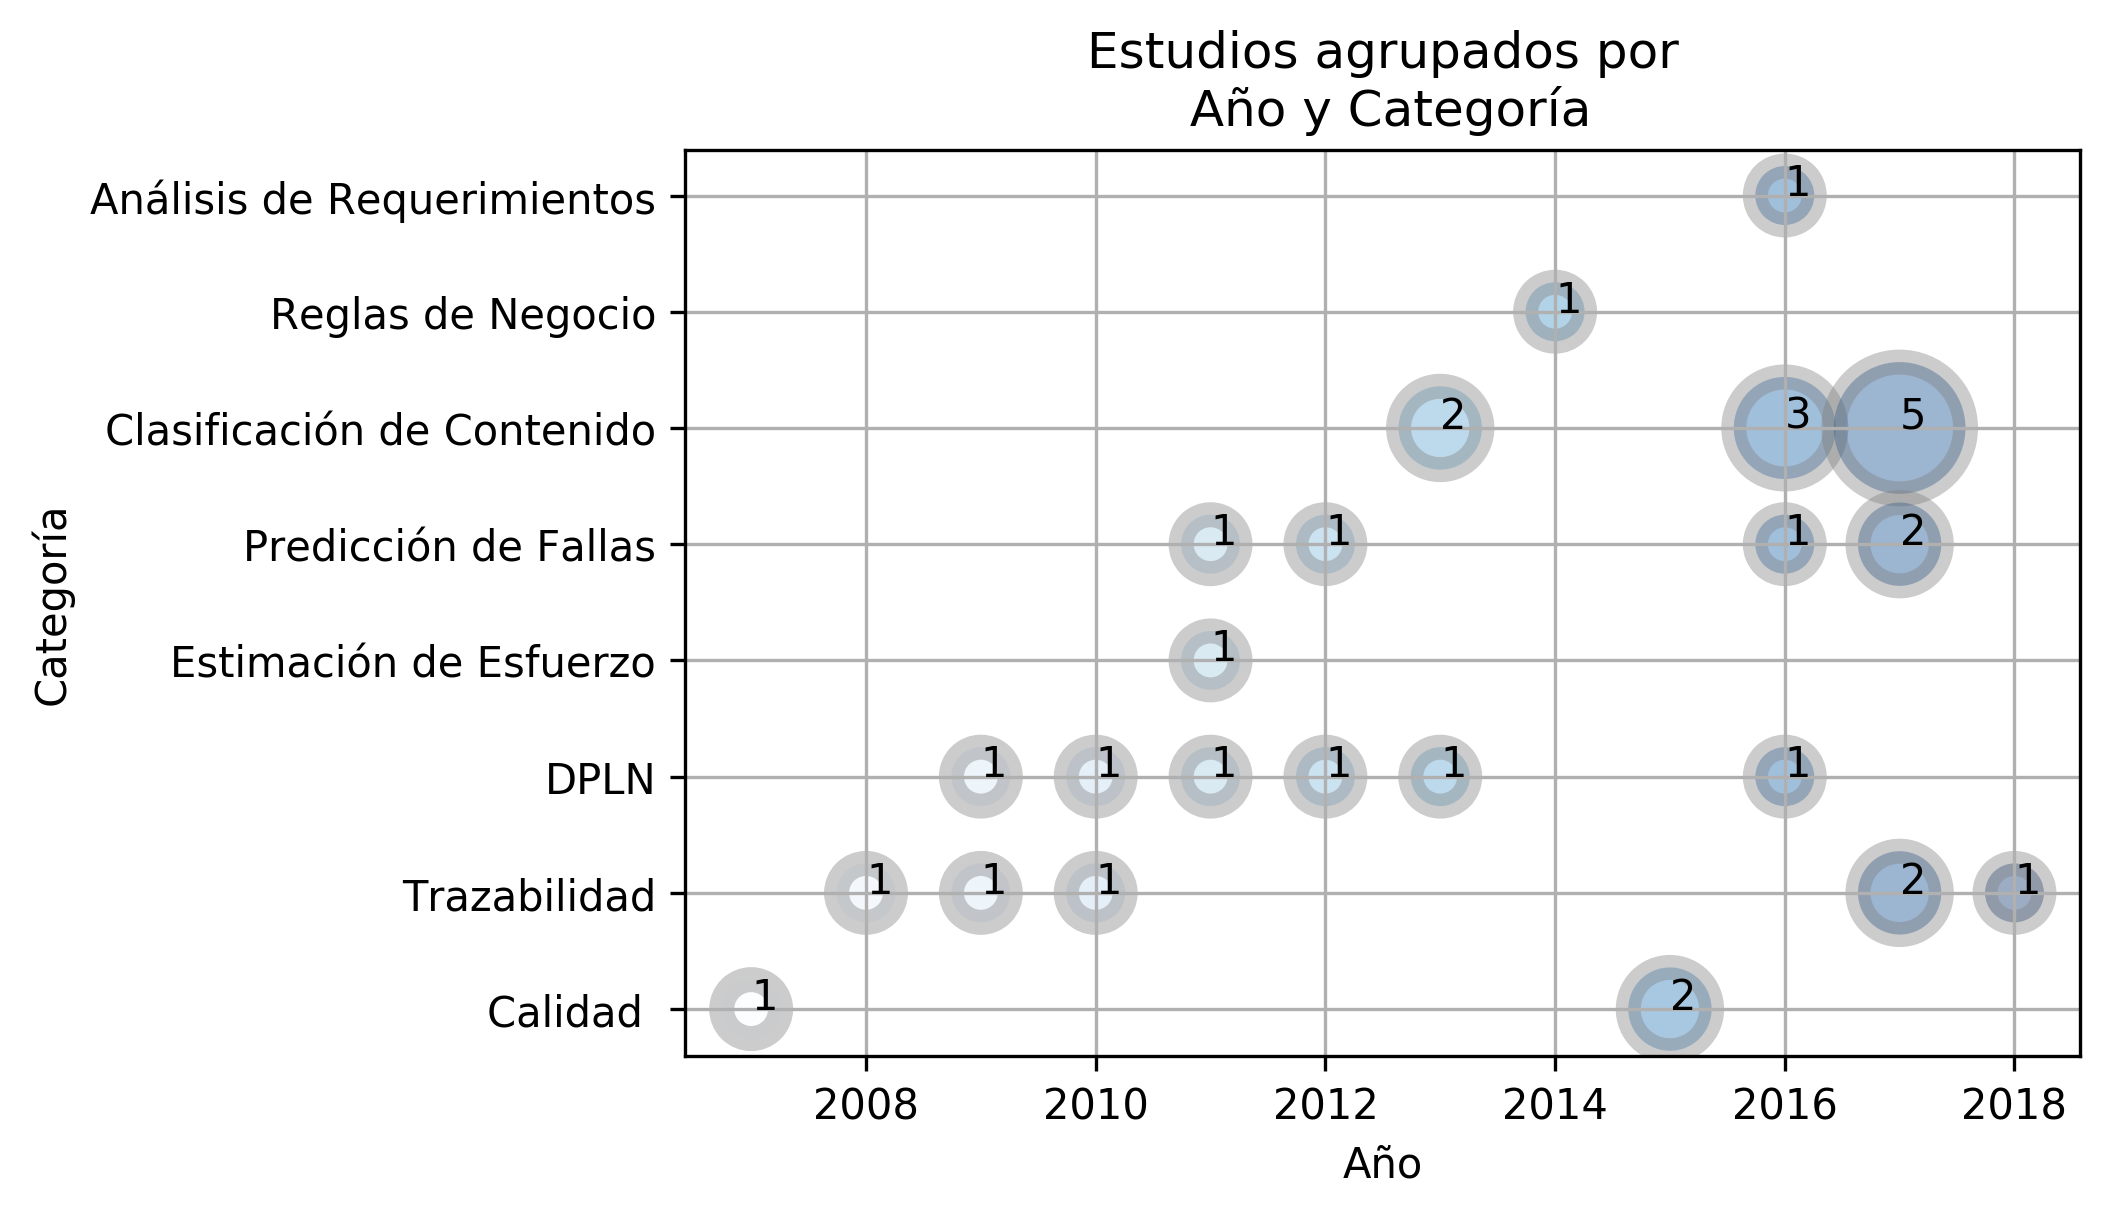
\includegraphics[width=3.2in]{figures/Figure8_Guada.png}
\caption{Distribución de artículos por año y categoría.}
\label{fig:8}
\end{figure}


\begin{figure}[!t]
\centering
\includegraphics[width=3.5in]{figures/figure9_Guada.png}
\caption{Relación entre algoritmos de AA y actividades de la IR.}
\label{fig:9}
\end{figure}

\begin{figure}[!t]
\centering
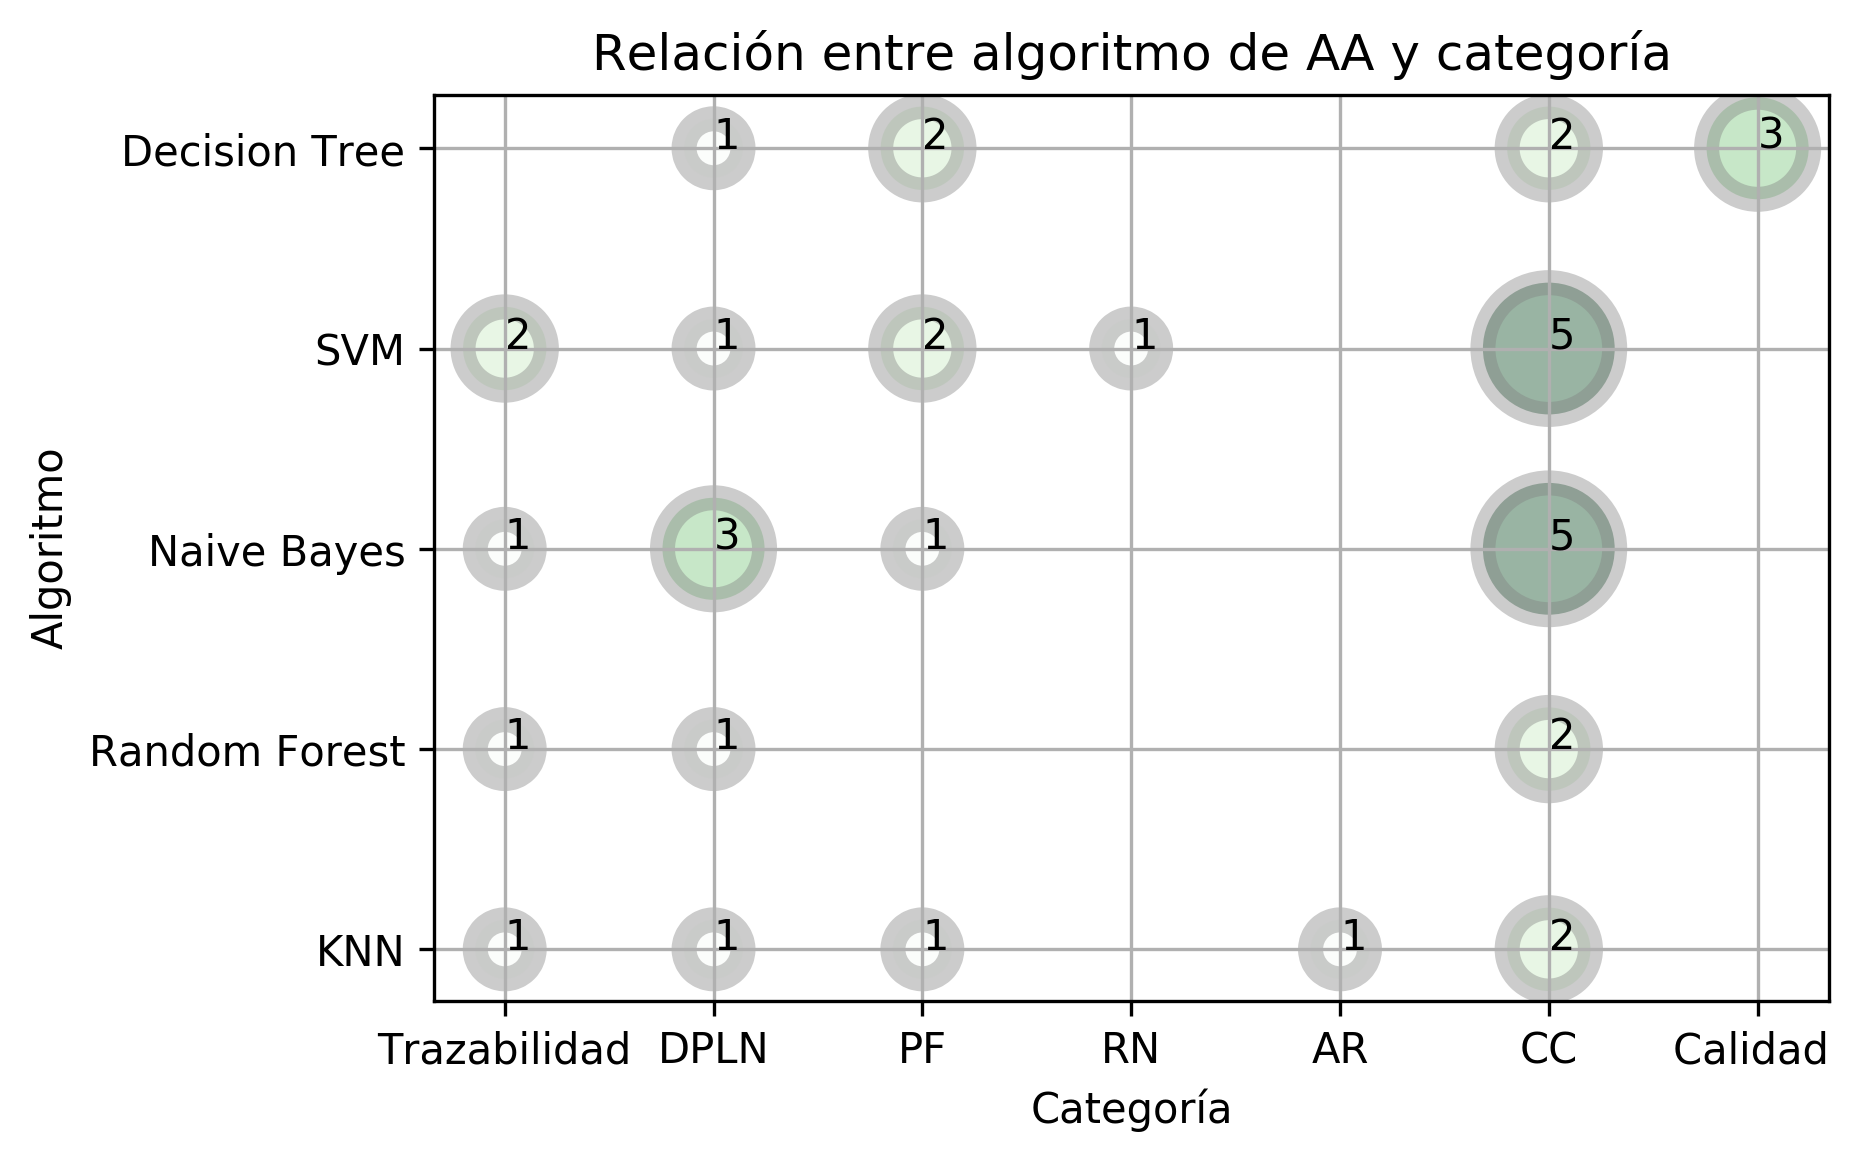
\includegraphics[width=3.5in]{figures/Figure11_Guadab.png}
\caption{Relación entre algoritmo de AA y categoría.}
\label{fig:10}
\end{figure}


La revisión comprensiva de los estudios seleccionados demuestra que las técnicas de aprendizaje supervisado en la IR se centran en ocho grandes categorías: (a) Análisis de requerimientos; (b) Identificación de reglas de negocio; (c) Detección de fallas; (d) Estimación del esfuerzo; (e) Resolución de problemas lingüísticos en documentos de requerimientos y artefactos escritos en lenguaje natural (PDNL); (f) Trazabilidad; y (g) Calidad. La Tabla \ref{tabla3} mapea los artículos identificados con las actividades de la IR y su correspondiente categoría asociada. 

En la Tabla \ref{tabla3}, se puede observar que las categorías clasificación de contenido, PDNL y trazabilidad, poseen una mayor cantidad de propuestas que aplican métodos de AA. Consecuentemente, es posible determinar que las actividades de la IR de mayor interés y experiencia respecto a la utilización de dichas técnicas corresponden al análisis de requerimientos, validación y verificación. 

La Fig. \ref{fig:8} muestra la distribución de artículos que emplean el aprendizaje supervisado en función a las categorías definidas.

En la Fig. \ref{fig:8} es posible apreciar que a pesar de la liberación en el año 2002 de librerías y nuevas tecnologías que permitieron explorar el uso de las técnicas de AA en diversos dominios, recién a partir del año 2006 comenzaron a ser aplicadas en el área de la IR. Las propuestas iniciales, estuvieron orientadas a la resolución de desafíos relacionados a la calidad y trazabilidad de los requerimientos. Sin embargo, las investigaciones sobre estas temáticas no mostraron grandes variaciones a largo del tiempo. 

Por otro lado, los estudios que abordaron la clasificación de contenidos en los documentos de requerimientos muestran mayor crecimiento entre los años 2016 y 2017. También cabe destacar, que la detección de problemas lingüísticos en documentos y artefactos escritos en lenguaje natural resultó ser uno de los retos más abordados hasta el año 2013.

A fin de proporcionar un mayor entendimiento e identificar tendencias respecto al uso de los métodos de AA, la Fig. \ref{fig:9} presenta la relación entre las actividades de la IR y los algoritmos de AA aplicados en las propuestas identificadas.

En la Fig. \ref{fig:9}, es posible apreciar los diez (10) algoritmos de AA más frecuentemente aplicados, en relación, a las actividades de la IR que presentan mayor cantidad de publicaciones. Consecuentemente, se observa que durante la actividad análisis de requerimientos, a menudo se aplican los algoritmos NB, SVM y KNN. Mientras que, en las actividades de validación y verificación de requerimientos las propuestas identificadas hacen uso de los algoritmos NB, SVM y DT. Por último, durante la especificación de requerimientos los algoritmos SVM y DT son los algoritmos aplicados con mayor frecuencia.  
Por otro lado, se observa que el  análisis de requerimientos es la actividad de la IR que presenta una variedad superior de algoritmos aplicados, en relación, a las actividades de validación verificación y especificación de requerimientos.  


\emph{\textbf{Q2. ¿Cuáles son los algoritmos de aprendizaje supervisado utilizados para resolver dificultades en las actividades de la IR?}}

Una amplia variedad de algoritmos de AA fueron detectados durante el análisis de las propuestas halladas en la literatura, éstos son utilizados para automatizar y optimizar las actividades involucradas en la IR. Fueron identificados cincuenta y cinco (55) algoritmos en los estudios seleccionados. El Anexo A presenta los algoritmos identificados por estudio.

Con el propósito de identificar los algoritmos más utilizados, la Fig. \ref{fig:10} muestra los cinco algoritmos de AA con mayor frecuencia de aplicación, en relación, a las cinco categorías que presentan mayor cantidad de propuestas. Las técnicas más utilizadas corresponden a NB, SVM, DT, KNN y Random Forest.

El algoritmo NB es aplicado en propuestas orientadas a la clasificación de contenido de los documentos de requerimientos (CC), detección y resolución de problemas lingüísticos en documentos y artefactos escritos en lenguaje natural (DPLN). Mientras que, es usado con menor frecuencia en tareas relacionadas a la trazabilidad y predicción de fallas (PF). 
Por lo que podemos concluir que dada la simplicidad que ofrece el algoritmo NB para construir modelos con un buen rendimiento, éste es usado en un amplio abanico de tareas y desafíos de la IR. 

El algoritmo SVM ha sido utilizado para abordar desafíos relacionados a la clasificación de texto y contenido de los documentos de requerimientos (CC), trazabilidad y predicción de fallas (PF). Posiblemente la selección de dicho algoritmo se deba a su efectividad en la resolución de tareas que involucren la categorización de entidades. También, fueron detectadas investigaciones que analizan la aplicación del algoritmo SVM en propuestas relacionadas a la trazabilidad. 

El algoritmo DT es utilizado para clasificar el contenido de los documentos (CC), predicción de fallas (PF) y en actividades relacionadas a la calidad de los requerimientos. Posiblemente la aplicación de este algoritmo se debe a su capacidad para representar y categorizar ciertas condiciones que ocurren en forma sucesiva a fin de resolver un problema determinado. Este algoritmo facilita la interpretación de los datos, dado que provee una visión gráfica de la toma de decisión necesaria, las variables evaluadas, las acciones que deben ser tomadas y el orden en la cual la toma de decisión será efectuada. 

El algoritmo KNN ha sido aplicado en actividades relacionadas a la clasificación de contenido (CC), trazabilidad, detección de problemas lingüísticos (DPLN), predicción de fallas (PF) y análisis de requerimientos (AR), lo cual evidencia su amplia flexibilidad y facilidad de aplicación.

Por último, el algoritmo Random Forest es utilizado frecuentemente para resolver problemas relacionados a la clasificación de contenido (CC) y en menor medida en propuestas que abordan la trazabilidad de requerimientos y detección de problemas lingüísticos en documentos de requerimientos y artefactos de escritos en lenguaje natural (DPLN). 

Resulta clave destacar que los estudios analizados no detallan una justificación respecto a los algoritmos aplicados. Y además, aproximadamente el 62\% de los estudios identificados utilizaron más de un algoritmo en sus propuestas de investigación, con la intención de seleccionar aquel que retorna mayor rendimiento. Esto denota la necesidad de un método formal que sirva de guía al proceso de selección de algoritmos de AA para ser aplicados en el área de IR.

\begin{figure}[!t]
\centering
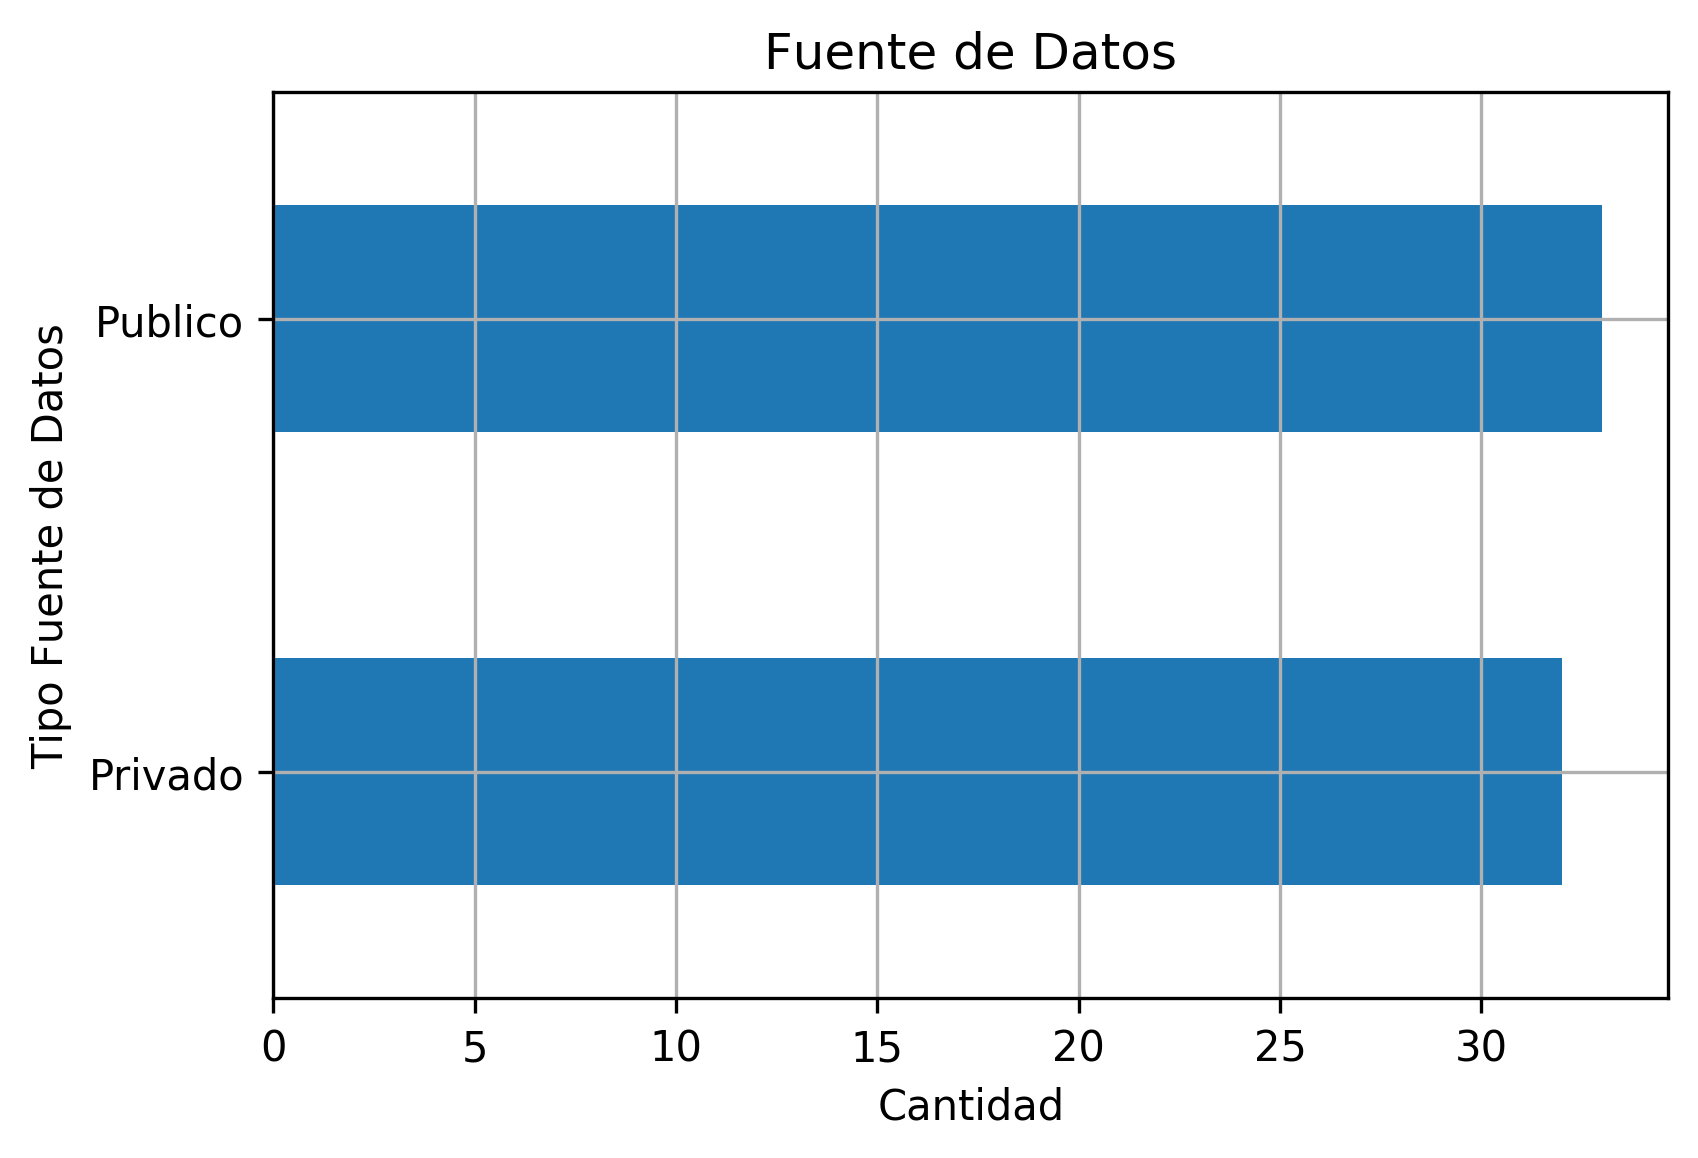
\includegraphics[width=3.5in]{figures/Figure10_Guada.png}
\caption{Cantidad de fuentes de datos públicas y privadas en total.}
\label{fig:11}
\end{figure}

\begin{figure}[!t]
\centering
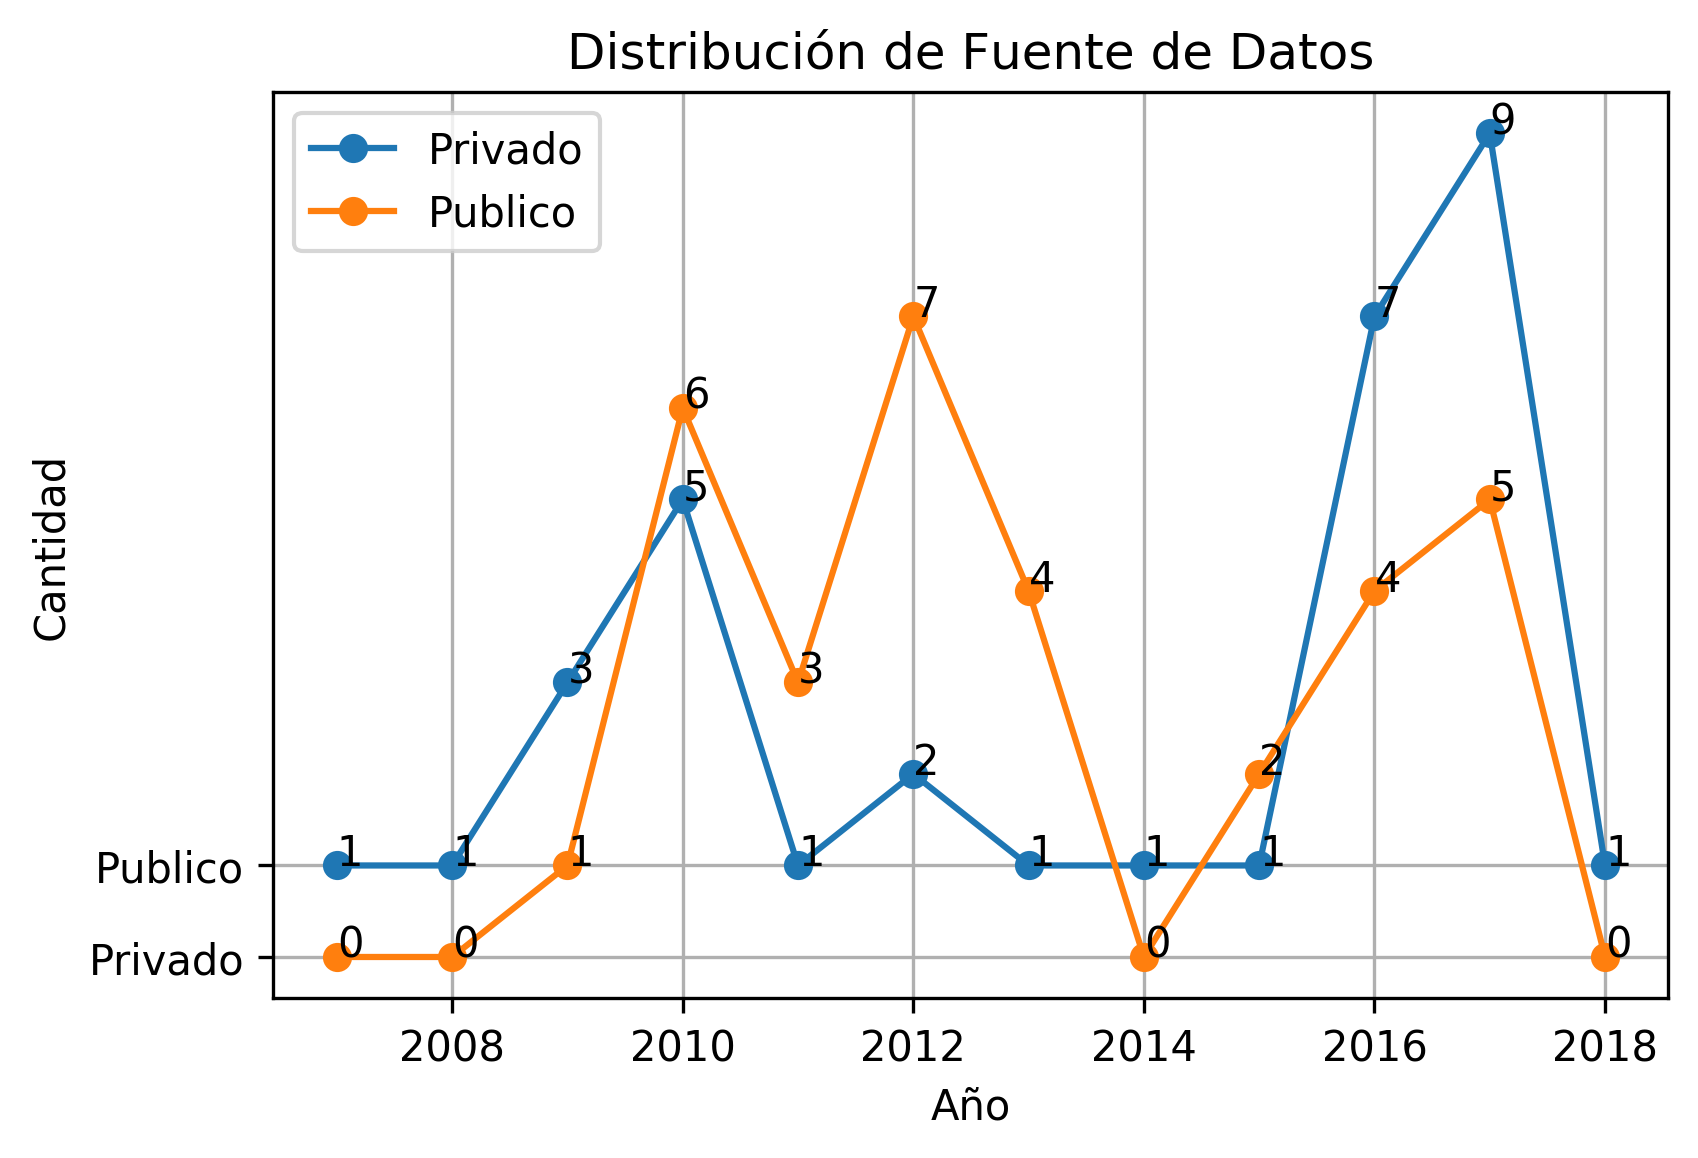
\includegraphics[width=3.5in]{figures/Figure12_Guada.png}
\caption{Distribución de fuentes de datos públicas y privadas.}
\label{fig:12}
\end{figure}

\emph{\textbf{Q3. ¿Cuáles son las principales fuentes de datos utilizadas para ejecutar los algoritmos de aprendizaje supervisado?} } 

En los estudios seleccionados, se han detectado diversas fuentes de datos, las cuales se clasificaron como públicas o privadas. Las fuentes de datos públicas están disponibles en repositorios y se distribuyen libremente. Mientras que las fuentes de datos privadas no son compartidas por los investigadores y, consecuentemente, resulta compleja la reproducción de sus propuestas. La Fig. \ref{fig:11} muestra la cantidad de fuentes de datos públicas y privadas identificadas.

A partir de los estudios analizados se identificaron veinticinco (25) fuentes de datos públicas y veintiocho (28) privadas. Entre las fuentes de datos públicas utilizadas con mayor frecuencia se encuentra PROMISE (Predictor Models In Software Engineering) utilizado en seis (6) estudios \cite{Jindal20162027,dekhtyar2017re,abad2017works,Slankas2013,fitzgerald2012early,malhotra2017exploratory}, cuatro (4) estudios utilizaron la fuente de datos iTrust Electronic Health Care System \cite{Slankas2013,Slankas2013a,winkler2016automatic,sharma2014automated} y dos (2) estudios \cite{fitzgerald2012early}, \cite{malhotra2017exploratory} utilizaron el repositorio MDP (Metric Data Program) de la NASA. Cabe señalar que hay algunos estudios que utilizaron más de un conjunto de datos para validar sus propuestas. La Fig. \ref{fig:12} muestra la distribución de las fuentes de datos privadas y públicas a lo largo de los años 2002-2018, considerados en este trabajo.

El empleo de fuentes de datos públicas y privadas en las diversas propuestas de investigación han presentado variaciones a lo largo de los años. Se observa que en período 2016-2017, han aumentado las propuestas que utilizan conjuntos de datos privados, probablemente consecuencia de la competencia global entre organizaciones. Sin embargo, el uso de conjuntos de datos públicos sigue siendo considerablemente elevado. Durante el período 2010-2012, la tendencia del uso de repositorios públicos ha sido notable. El Anexo A mapea las fuentes de datos utilizadas por estudio.

Como se mencionó en secciones anteriores, el AA utiliza conjuntos de datos para entrenar un modelo y en base a ello hacer predicciones útiles. Es por esta razón, es necesario destacar que el uso de conjuntos de datos públicos permite que las investigaciones propuestas sean repetibles, refutables y verificables \cite{Catal2009} proporcionando de esta manera, valor a la comunidad científica para encarar futuras investigaciones. En relación a esto, en la década de 1990, se creó un repositorio llamado UCI \footnote{https://archive.ics.uci.edu/ml/index.php} (University of California Irvine) como un servicio a la comunidad que utiliza el AA, el cual actualmente posee 468 conjuntos de datos. 

Inspirados en el esfuerzo de la UCI, posteriormente, los investigadores involucrados en el área de Ingeniería de Software desarrollaron el repositorio PROMISE\footnote{http://promise.site.uottawa.ca/SERepository}, que cuenta con numerosos conjuntos de datos públicos desde el año 2005. El repositorio PROMISE fue creado para fomentar modelos predictivos repetibles, verificables, refutables y/o mejorables, lo que resulta esencial para la madurez de cualquier disciplina de investigación. 

Otra de las fuentes de datos disponibles es MDP de la NASA \footnote{http://mdp.ivv.nasa.gov}, que actualmente consta de 13 conjuntos de datos destinados explícitamente a la investigación de métricas de software. Cada conjunto de datos representa un sistema/subsistema de software de la NASA, contiene las métricas de código y los datos respecto a las fallas de cada módulo que lo compone.

Por otro lado, iTrust\footnote{https://bensmith.s3.amazonaws.com/website/papers/sst2011.pdf} es un proyecto de software de código abierto, su objetivo es el desarrollo de una aplicación médica que mantiene el registro de los pacientes y su historial médico, además, permitir la comunicación entre médicos. La documentación del proyecto consiste en 59 casos de uso y 11 módulos de código, todos sus artefactos se encuentran disponibles en línea públicamente. 

\section{ANÁLISIS Y DISCUSIONES DE LOS RESULTADOS}

En esta investigación se analizan los estudios que aplican técnicas de aprendizaje supervisado para resolver dificultades en la IR. Como resultado del proceso de análisis, se observó la existencia de artículos que utilizan un conjunto de algoritmos para entrenar sus modelos y luego comparar su rendimiento, los artículos identificados fueron dieciocho (18).

Especialmente, se destaca la propuesta de Nikora y Balcom \cite{nikora2009automated} quienes emplean un conjunto de treinta y un (31) algoritmos utilizando la herramienta WEKA.

Por otro lado, se detectó que los algoritmos SVM y NB en combinación con las técnicas de procesamiento de lenguaje natural son utilizados para resolver problemas relacionados a aspectos lingüísticos en documentos de requerimientos escritos en lenguaje natural y clasificación de contenido. Las ANN fueron utilizadas para eliminar la necesidad de extracción manual de características en los documentos de requerimientos. Para abordar problemas de clasificación fueron utilizados los algoritmos DT, KNN y Regression Logistic (algoritmos clasificadores). Mientras que, las técnicas de ensamblado, tales como Bagging y Boosting fueron los algoritmos usados en menor medida debido a que requieren para su entrenamiento grandes conjuntos de datos. En este sentido, Ott \cite{Ott2013} destaca la necesidad real de continuar trabajando e impulsando el uso de datos públicos en las investigaciones, a fin de disponer de conjuntos de datos de mayor volumen para el entrenamiento de los algoritmos, pilar fundamental del campo del AA. 

Entre las actividades de la IR más abordadas se identifican el análisis, especificación, validación y verificación de requerimientos. Consecuentemente, es posible determinar que las actividades relacionadas a la obtención y extracción de requerimientos constituyen una laguna de investigación en el área. 

Otro aspecto para destacar es la gran variedad de algoritmos aplicados en las propuestas de investigación, lo que denota la necesidad de un procedimiento o consideraciones formales que faciliten el proceso de selección de los mismos para su aplicación en el área de requerimientos. Aún más, no se halló evidencia de una hoja de ruta formalmente documentada que especifique las condiciones necesarias para aplicar las técnicas de AA en el campo de la IR. En relación a las pautas necesarias para la preparación de las fuentes de datos para su posterior procesamiento, tampoco se halló evidencia. Esta situación, demuestra la necesidad de procesos y/o consideraciones formales en dicha área de investigación. 

La Fig. \ref{fig:13} ofrece un mapa mental que resume los algoritmos más frecuentemente usados, las tareas de la IR en las que se aplican las técnicas de aprendizaje supervisado y las fuentes de datos públicas más utilizadas en los artículos. Además, las revistas y conferencias más significativas en el área también fueron consideradas. 

Durante el desarrollo de esta investigación, no se abordaron ciertas temáticas de interés dada la exhaustividad que requiere su análisis, pero sin duda valen la pena su estudio y discusión en trabajos posteriores. Este artículo no aborda un análisis comparativo respecto al rendimiento de los algoritmos de AA aplicados en la resolución de un mismo problema o actividad de la IR. El flujo o metodología de trabajo utilizado en las propuestas de investigación para aplicar los modelos de AA, no fueron discutidos. Sin embargo, resulta fundamental determinar las metodologías de trabajo utilizadas, a fin de identificar posibles patrones de aplicación.  Por último, en este trabajo no es evaluado el impacto y el nivel de aceptación de las industrias que apuestan a la implementación de propuestas que utilizan técnicas de AA. 

\section{AMENAZAS A LA VALIDEZ}

En esta sección se discuten las posibles amenazas a la validez respecto a los resultados obtenidos durante el proceso de revisión de los artículos seleccionados. El mapeo sistemático propuesto ofrece un estudio de las investigaciones en el área de la IR que aplican técnicas de aprendizaje automático supervisado para resolver diversas tareas y desafíos. A pesar de los esfuerzos de los autores para disminuir los sesgos respecto a la selección de los artículos y resultados obtenidos, existen potenciales amenazas que podrían afectar su validez. Las posibles amenazas identificadas en esta investigación están representadas por el sesgo en la selección de estudios incluidos, la extracción de datos de diferentes fuentes y la síntesis de datos. Para mitigar las amenazas potenciales a la validez, se aplicó un protocolo de investigación definido y reconocido por la comunidad científica para realizar estudios de mapeo. Tal como proponen Petersen y otros \cite{petersen2008systematic}, este protocolo propone la definición de preguntas de investigación, criterios de inclusión/exclusión y una estrategia de investigación. Además, se analizaron y debatieron los términos incluidos en la cadena de búsqueda de acuerdo al ámbito de interés de los autores en la temática.

Posteriormente, se realizaron pruebas piloto de la cadena de búsqueda para comprobar el alcance definido en esta investigación. Durante el proceso de revisión, todos los autores experimentados en el área participaron y debatieron en  la toma de decisiones acerca de los documentos incluidos en el estudio.


\begin{figure}[!t]
\centering
\includegraphics[width=3.5in]{figures/figure13_Guada.png}
\caption{Mapa mental resultante del mapeo sistemático de la literatura.}
\label{fig:13}
\end{figure}

Otro de los posibles sesgos presente en la investigación está relacionado con la inclusión de artículos redactados sólo en inglés, dado el bajo nivel de difusión de publicaciones y artículos redactados en otros idiomas, en revistas relevantes de Ingeniería de Software. Cabe destacar, que los autores definieron este criterio considerándolo además, como un límite del alcance de la investigación propuesta. En particular, no se propuso un procedimiento para mitigar este posible sesgo, sino que fue  planteado como una futura línea de investigación.  

Por otro lado, es necesario considerar que los resultados obtenidos pueden variar en relación a la fecha de ejecución de la cadena de búsqueda y respecto a los accesos a las bibliotecas científicas digitales otorgados a las Universidades e Instituciones de pertenencia de los autores. Consecuentemente, esta situación puede conducir a otro posible sesgo en la investigación dada la no inclusión de algunas bibliotecas relevantes.


\section{CONCLUSIONES}

El mapeo sistemático de la literatura propuesto tiene como objetivo identificar y analizar tendencias, conjuntos de datos y métodos de aprendizaje supervisado utilizados para resolver tareas y desafíos presentes en la IR entre los años 2002 y 2018.

Considerando los criterios de inclusión y exclusión definidos, se analizaron treinta y tres (33) estudios publicados en revistas y conferencias significativas en el área de Ingeniería de Software. El análisis de los estudios seleccionados reveló que las técnicas de aprendizaje supervisado pueden ser aplicadas para resolver y automatizar tareas relacionadas con la IR, enfocándose principalmente en ocho categorías: detección de problemas lingüísticos en documentos de requerimientos y artefactos escritos en lenguaje natural, clasificación de contenido de documentos, trazabilidad, estimación del esfuerzo, análisis de requerimientos, predicción de fallas, calidad y detección de reglas de negocio.

En esta investigación, se detectaron cincuenta y cinco (55) algoritmos aplicados en las diversas propuestas. Los cinco algoritmos más aplicados son NB, SVM, DT, KNN y Random Forest.
En relación a las fuentes de datos utilizadas para entrenar los modelos de AA propuestos, se identificaron veinticinco (25) fuentes de datos públicas y veintiocho (28) privadas. Las fuentes de datos públicas utilizadas con mayor frecuencia fueron PROMISE, iTrust Electronic Health Care System y MDP,  aplicados en seis (6), cuatro (4) y dos (2) estudios respectivamente. Es necesario destacar, la presencia de algunos estudios que utilizaron más de un conjunto de datos para validar sus modelos. 

Los resultados obtenidos en esta investigación permiten evidenciar el valor de los algoritmos de aprendizaje supervisado en el área de la IR. Dado que, tal como los demuestran las propuestas analizadas éstos permiten la optimización y automatización de las actividades involucradas. Aún más, es necesario destacar que no se encontraron trabajos que desestimen la aplicación de las técnicas de AA en la obtención de mejoras y resolución de problemas en dicha área de investigación. Este hecho demanda la necesidad de continuar indagando acerca de sus beneficios y usos posibles.

Adicionalmente, se identificaron lagunas de investigación también, específicamente en tareas relacionadas a la obtención y extracción de requerimientos, las cuales son fundamentales para el éxito de un proyecto de software. Consecuentemente, este hecho representa una oportunidad de investigación en el área, por lo que  las contribuciones y mejoras que se puedan realizar favorecerán a todo el ciclo de vida del software.  

Los autores proponen como futura línea de investigación la definición de un proceso formal que sirva de guía para la elección de algoritmos de AA, de acuerdo al tipo de problema o tarea que se desea resolver en la IR, basado en las experiencias y estudios analizados. Y, por último, extender la investigación al análisis de estudios y propuestas redactados en otros idiomas.   

% use section* for acknowledgment
\section*{Agradecimientos}

Los autores agradecen el apoyo brindado por las siguientes instituciones: CONICET y Universidad Tecnológica Nacional (SIUTIFE0004923TC).


% Can use something like this to put references on a page
% by themselves when using endfloat and the captionsoff option.
\ifCLASSOPTIONcaptionsoff
  \newpage
\fi

% trigger a \newpage just before the given reference
% number - used to balance the columns on the last page
% adjust value as needed - may need to be readjusted if
% the document is modified later
%\IEEEtriggeratref{8}
% The "triggered" command can be changed if desired:
%\IEEEtriggercmd{\enlargethispage{-5in}}

% references section

% can use a bibliography generated by BibTeX as a .bbl file
% BibTeX documentation can be easily obtained at:
% http://mirror.ctan.org/biblio/bibtex/contrib/doc/
% The IEEEtran BibTeX style support page is at:
% http://www.michaelshell.org/tex/ieeetran/bibtex/
%\bibliographystyle{IEEEtran}
% argument is your BibTeX string definitions and bibliography database(s)
%\bibliography{IEEEabrv,../bib/paper}
%
% <OR> manually copy in the resultant .bbl file
% set second argument of \begin to the number of references
% (used to reserve space for the reference number labels box)

\bibliographystyle{ieeetr}
\bibliography{referencia1}

\small
\onecolumn
\begin{longtable}[c]{p{0.50cm}p{4.5cm}p{2.5cm}p{2.5cm}p{2.5cm}}
\caption{ANEXO A}
\label{tablaA} \\
\hline
\hline
ID & Resumen & Categoría & Algoritmo & Fuente de Datos \\
\hline
\cline{1-5}
\cite{Li201725} & Li y otros proponen un enfoque basado en ontologías para predecir la trazabilidad de los requerimientos y utilizan el algoritmo Support Vector Machine para entrenar los datos. & Trazabilidad & Support Vector Machine & Pine System\\ \cline{1-5}

\cite{yang2010extending} & Yang y otros proponen desarrollar un sistema para clasificar automáticamente las ambigüedades en los requerimientos redactados en lenguaje natural, como nocivos o inofensivos, e informar al analista de los casos potencialmente peligrosos. Desarrollaron un clasificador utilizando técnicas de aprendizaje automático, específicamente Naives Bayes. Los autores destacan la necesidad de un conjunto de datos más grande para mejorar la precisión de la predicción. & Problemas lingüísticos en documentos de requerimientos y artefactos escritos en lenguaje natural & Naive Bayes & RE\@UTS \\ \cline{1-5}

\cite{yang2012speculative} & Yang y otros presentan un enfoque para detectar automáticamente la incertidumbre sobre los requerimientos expresados en lenguaje natural. El enfoque aplicado consta de dos etapas. En la primera los autores identifican frases especulativas mediante la aplicación de campos aleatorios condicionales (CRF). Mientras que en la segunda etapa utilizan un conjunto de heurísticas lingüísticas para determinar el nivel de incertidumbre alcanzado en las oraciones analizadas. & Problemas lingüísticos en documentos de requerimientos y artefactos escritos en lenguaje natural & Conditional Random Field & RE\@UTS \\ \cline{1-5}

\cite{Knauss201685} & Knauss y otros proponen ACon (Adaptation of Contextual Requirements), un proyecto para abordar la incertidumbre que afecta a los requerimientos en tiempo de ejecución. ACon utiliza un bucle de retroalimentación para detectar las necesidades contextuales afectadas por la incertidumbre e integra el algoritmo JRip (un clasificador basado en reglas) para analizar y determinar el contexto en el cual los requisitos son válidos. & Problemas lingüísticos en documentos de requerimientos y artefactos escritos en lenguaje natural & Jrip & TOTEM \\ \cline{1-5}

\cite{Yang2011} & Yang y otros describen un enfoque para identificar automáticamente ambigüedades potencialmente nocivas, centrándose en la ambigüedad anafórica, que ocurre cuando los lectores no están de acuerdo en cómo deben interpretarse los pronombres en una oración. A través de la definición de heurísticas capturan información acerca de los aspectos que pueden llevar a un lector a una interpretación particular del texto. A partir de estas heurísticas construyen un clasificador utilizando los algoritmos Naives Bayes y K- Nearest Neighbor para predecir las interpretaciones del lector. & Problemas lingüísticos en documentos de requerimientos y artefactos escritos en lenguaje natural & K- Nearest Neighbor; Naive Bayes & RE\@UTS \\ \cline{1-5}

\cite{Ott2013} & Ott propone un método para detectar defectos de consistencia o integridad, entre los requerimientos de software utilizando algoritmos de clasificación de texto. Se evaluaron dos algoritmos de clasificación, Multinomial Naive Bayes (MNB) y Support Vector Machine (SVM). Para validar la propuesta se utilizaron dos especificaciones automotrices de Mercedes-Benz.  El autor destaca la necesidad de continuar trabajando para mejorar la adquisición de datos de entrenamiento (mayor volumen). & Problemas lingüísticos en documentos de requerimientos y artefactos escritos en lenguaje natural & Multinomial Naive Bayes; Support Vector Machine & Mercedes Benz  \\ \cline{1-5}

\cite{nikora2009automated} & Nikora y Balcom proponen aplicar aprendizaje automático para identificar tipos específicos de requerimientos redactados en lenguaje natural dentro de un conjunto de especificaciones. En este caso, se evaluaron treinta y un (31) algoritmos de clasificación sobre el conjunto de datos de entrenamiento, utilizando la herramienta WEKA. Los resultados en esta investigación demuestran que no hay una diferencia significativa en cuanto al rendimiento de los algoritmos utilizados. & Problemas lingüísticos en documentos de requerimientos y artefactos escritos en lenguaje natural & AD Tree; Bayes Network; Complement Naives Bayes; Conjunctive Rule; Decision Stump; Decision Table; Hyper Pipes; IB1; Ibk ; Decision Tree; Jrip;  Kstar, LMT; Simple Logistic;  LWL;  Multilayer Perceptron;  Naive Bayes Multinomial;  Naive Bayes Updateable;  Naive Bayes, NB Tree;  Nnge; OneR; PART; Random Forest;   Random Tree; RBF Network;  Ridor ; Sequential minimal optimization; VFI;  Voted Perceptron;  Zero R & Jet Propulsion Laboratory (JPL) \\ \cline{1-5}

\cite{li2017identifying} & Li propone un método basado en técnicas de aprendizaje automático y análisis lingüístico para identificar requerimientos de seguridad. Este trabajo utiliza cuatro tipos de algoritmos, incluyendo los basados en Bayes, árboles, funciones y reglas. El autor tomó dos algoritmos de cada uno de estos tipos respectivamente, Naive Bayes (NB), BayesNet (BN), Logistic Model Tree (LMT), J48, Sequential minimal optimization (SMO), Logistic, Decision Table (DT) y PART & Clasificación de Contenido & Naive Bayes; BayesNet, Logistic Model Tree; J48; Sequential minimal optimization; Logistic; Decision Table; PART & CEPSCO; TISPAN; Global Platform \\ \cline{1-5}

\cite{Jindal20162027} & Jindal y otros proponen extraer las descripciones de requisitos de seguridad presentes en los documentos de requerimientos (ERS) y desarrollar un modelo de clasificación utilizando el algoritmo árbol de decisión J48. Esta propuesta es evaluada con las especificaciones de requerimientos procedentes de 15 proyectos desarrollados por estudiantes de la Universidad De Paul disponibles públicamente en el repositorio PROMISE. & Clasificación de Contenido & Decision Tree (J48) & Predictor Models In Software Engineering (PROMISE) \\ \cline{1-5}

\cite{kurtanovic2017automatically} & Kurtanović y Maalej investigan sobre la precisión con la cual es posible clasificar automáticamente los requerimientos como funcionales (RF) y no funcionales (RNF). Para ello, evaluaron los algoritmos Support Vector Machine, Adaptive Boost, Gradient Boosting y Gradient Boosting. & Clasificación de Contenido & Support Vector Machine; Adaptive Boost; Extra-Trees; Gradient Boosting; Random Forest & Amazon \\ \cline{1-5}

\cite{dekhtyar2017re} & Dekhtyar y Fong presentan un enfoque para clasificar los RNF utilizando Word2vec, Convolutional Neuronal Network y Naive Bayes. & Clasificación de Contenido & Naive Bayes; Word2Vec; Convolutional Neuronal Network & PROMISE; Fachgebiet Software Engineering \\ \cline{1-5}

\cite{abad2017works} & Abad y otros proponen un enfoque de pre-procesamiento que estandariza y normaliza los requerimientos antes de aplicar algoritmos de clasificación. Además, los autores investigan sobre diversos algoritmos (Decision Tree, Latent Dirichlet Allocation, Naive Bayes) para clasificar de manera automática los RNF. & Clasificación de Contenido & Decision Tree; Latent Dirichlet Allocation; K-means; Naive Bayes &  PROMISE \\ \cline{1-5}

\cite{Slankas2013} & Slankas y Williams proponen extraer y categorizar los RNF a partir de la documentación disponible (acuerdos de uso, manuales de instalación, reglamentos, especificaciones de requerimientos y manuales de usuario) mediante procesamiento de lenguaje natural y aprendizaje automático. En esta propuesta se utiliza K-Nearest Neighbor, Naive Bayes, Support Vector Machine, Sequential Minimal Optimization (SMO) y para agrupar las oraciones relacionadas utilizaron el algoritmo K-medois. & Clasificación de Contenido & K-medois; K- Nearest Neighbor; Naive Bayes; Support Vector Machine; Sequential minimal optimization & iTrust; Promise; CCHIT \\ \cline{1-5}

\cite{Slankas2013a} & Slankas y Williams proponen un proceso basado en técnicas de aprendizaje automático para analizar documentos escritos en lenguaje natural. El objetivo es extraer temas, acciones y recursos relevantes para la especificación de una política de control de acceso. El proceso utiliza una combinación de los algoritmos K-Nearest Neighbor, Naive Bayes y Support Vector Machine. También se utiliza el algoritmo de agrupamiento K-medois para agrupar las oraciones relacionadas. & Clasificación de Contenido & K-Nearest Neighbor; Naive Bayes; Support Vector Machine; K-medois & iTrust \\ \cline{1-5}

\cite{Merten2016} & Merten y otros utilizan técnicas de procesamiento de lenguaje natural y aprendizaje automático para detectar requerimientos en los sistemas de seguimiento de problemas, para lo cual utilizaron las librerías NLTK y Scikit-learn. En esta propuesta se utilizaron siete (7) algoritmos de aprendizaje automático Naive Bayes; Multinomial Naive Bayes; Support Vector Machine; Logistic Regression; Stochastic Gradient Descent; Decision Tree; Random Forest. & Clasificación de Contenido & Naive Bayes; Naive Bayes Multinomial, Support Vector Machine; Logistic Regression; SGD (Descenso Gradiente Estocástico); Decision Tree; Random Forest & cgeo; Lighttpd; Radiant; Redmine \\ \cline{1-5}

\cite{winkler2016automatic} & Winkler y Vogelsang presentan un enfoque para clasificar automáticamente el contenido de una especificación de requerimientos como "requerimiento" o "información", utilizando redes neuronales convulatorias. & Clasificación de Contenido & Convolutional Neural Network & Mercedes Benz \\ \cline{1-5}

\cite{Cleland-Huang2010} & Cleland-Huang y otros presentan dos métodos de aprendizaje automático para mejorar la calidad de los enlaces de trazabilidad entre los requerimientos. Los autores utilizan un algoritmo de clasificación propio desarrollado en una investigación anterior & Trazabilidad & Propio & Care2x; CCHIT; Clear Health; Physician; iTrust; Trial Implementation; PatientOS; Practice One; Lauesen; World VistA \\ \cline{1-5}

\cite{gokyer2008non} & Gokyer y otros proponen un enfoque para extraer automáticamente aspectos arquitectónicos y atributos de calidad desde RNF expresados en texto plano. Para alcanzar dicho objetivo se utiliza el algoritmo Support Vector Machine y técnicas de procesamiento de lenguaje natural. & Trazabilidad & Support Vector Machine & Cybersoft \\ \cline{1-5}

\cite{Mills2017} & Mills y Haiduc proponen un enfoque predictivo que proporciona una clasificación booleana (es decir, válida o inválida) para todos los posibles vínculos o enlaces de trazabilidad entre los conjuntos de artefactos de software. El enfoque utiliza el clasificador de aprendizaje de automático Random Forest implementado en la herramienta Weka. & Trazabilidad & Random Forest & eAnci; eTour; SMOS \\ \cline{1-5}

\cite{Sardinha2013} & Sardinha y otros presenta EA-Analyzer, una herramienta automatizada para identificar dependencias conflictivas entre requerimientos en los documentos de especificación, utilizando el algoritmo Naive Bayes. & Trazabilidad & Naive Bayes & Health Watcher; Smart Home; CAS \\ \cline{1-5}

\cite{sharma2014automated} & Sharma y otros presentan un enfoque para la identificación de las reglas de negocio en los documentos de requerimientos. En esta propuesta se utilizaron los algoritmos Support Vector Machine, Naïve Bayes, BayesNet y Random Forest. & Reglas de Negocio & Support Vector Machine; Random Forest; Bayes Network; Naive Bayes & Propio \\ \cline{1-5}

\cite{Parra2015180} & Parra y otros proponen evaluar automáticamente la calidad de los requerimientos, emulando la evaluación que haría un experto en calidad de un proyecto. Los autores utilizan algoritmos de aprendizaje automático (Decision Tree, PART, Boosting, Bagging, Induction Rules) para generar clasificadores y predecir la calidad de los requisitos. & Calidad & Decision Tree; PART; Boosting, Bagging; Induction Rules & INCOSE \\ \cline{1-5}

\cite{Hayes2015} & Hayes y otros proponen utilizar los algoritmos Decision Tree y Logistic Regression para determinar si los requerimientos cumplen con los aspectos de calidad a fin de ser sometidos a las etapas de testing. & Calidad & Regression Logistic; Decision Tree & Browser; iTrust \\ \cline{1-5}

\cite{Hussain2007} & Hussain y otros aplican técnicas de aprendizaje automático (Decision Tree) para detectar especificaciones ambiguas en los documentos de requerimientos, considerando indicadores de calidad definidos en un modelo de calidad propuesto por los autores. & Calidad & Decision Tree & Designfest \\ \cline{1-5}

\cite{del2017stability} & Del Sagrado y Águila utilizan Bayesian Network para evaluar las especificaciones de requerimientos y determinar si cumplen con los atributos de calidad o requieren revisión. & Predicción de Fallas & Bayes Network & RALIC \\ \cline{1-5}

\cite{dargan2016systems} & Dargan y otros introducen un modelo estadístico utilizado para predecir el rendimiento operativo del sistema a partir de los requerimientos de calidad.  Esta propuesta evalúa los algoritmos Logistic Regression, Naive Bayes Classifier, Support Vector Machine y K-Nearest Neighbor para desarrrollar un modelo predictivo. & Predicción de Fallas & Naive Bayes; Support Vector Machine; K- Nearest Neighbor; Logistic Regression & ORD (Operational Requirements Document); KPPs (Key Performance Parameters); Operational Test Report \\ \cline{1-5}

\cite{fitzgerald2012early} & Fitzgerald y otros presentan un modelo de predicción de fallas relacionadas a las funcionalidades solicitadas durante la obtención de requerimientos. Esta propuesta emplea los algoritmos Decision Table, Naive Bayes, Linear Regression y M5P-Tree. & Predicción de Fallas & Naive Bayes; Lineal Regression; Decision Tree  & Eclipse; FireFox; KDE; Netbeans; Wikimedia; Thunderbird; Apache \\ \cline{1-5}

\cite{malhotra2017exploratory} & Malhotra y Khanna sostienen que la volatilidad de los requerimientos, actualización tecnológica y ocurrencia de los defectos requieren cambios en el software para su uso efectivo. Es por ello que proponen un enfoque para la predicción de clases en el código propensas al cambio. Esta propuesta utiliza Decision Tree, Support Vector Machine, CART y Multilayer Perceptron. & Predicción de Fallas  & Decision Tree; Support Vector Machine; CART; Multilayer Perceptron & Ice Cream Sandwich; Jelly Bean \\ \cline{1-5}

\cite{del2011requirement} & Águila y Del Sagrado proponen un modelo para predecir la ocurrencia de riesgos a partir de las métricas de requerimientos, utilizando Bayesian Network y Decision Tree. & Predicción de Fallas & Bayes Network; Decision Tree & PROMISE; MDP (Metrics Data Program) \\ \cline{1-5}

\cite{Abdukalykov2011158} & Abdukalykov y otros proponen utilizar técnicas de aprendizaje automático para estimar el esfuerzo del proyecto de software. El modelo propuesto se basa en datos históricos de proyectos anteriores y en base a ello, estima el esfuerzo de desarrollo durante la fase de especificación de requerimientos. Se utilizan K Nearest Neighbor y Linear Regression. & Estimación de Esfuerzo & Artificial Neuronal Network; Linear Regression & ISBSG COSMIC \\ \cline{1-5}

\cite{Wang2016} & Wang propone un enfoque para analizar automáticamente las especificaciones de los requerimientos de software y extraer la información semántica utilizando el algoritmo K-Nearest Neighbour. & Análisis de Requerimientos & K-Nearest Neighbour & Propio \\ \cline{1-5}

\cite{kurtanovic2017automatically} & Kurtanović y Maalej proponen un enfoque que utiliza metadatos, características léxicas y sintácticas para clasificar automáticamente RF y RNF (usabilidad, seguridad, funcionamiento y rendimiento). Para desarrollar esta propuesta utilizaron el algoritmo Support Vector Machine, alcanzando medidas de precisión (recall y precision) de aproximadamente el 92\% para ambas clases de requerimientos. El conjunto de datos utilizado corresponde a una muestra aleatoria de revisiones de software de Amazon (SR) rastreadas entre 2014 y 2016. & Clasificación de Contenido  & Support Vector Machine  & Amazon  \\ \cline{1-5}

\cite{AtasM.2018} & Atas y otros presentan un enfoque para identificar automáticamente las dependencias entre requerimientos mediante el uso de técnicas de clasificación supervisada. Se evaluaron los algoritmos Naive Bayes, Linear Support Vector Machine, K-Nearest Neighbors y Random Forest. Los resultados de esta propuesta demuestran que el algoritmo Random Forest puede detectar dependencias entre requerimientos con una calidad alta de predicción (aproximadamente 82\%). Para evaluar este enfoque se utiliza un conjunto de requerimientos derivados de un proyecto que tiene como objetivo el desarrollo de un reloj deportivo (smartwatch). & Trazabilidad  & Naive Bayes; Linear Support Vector Machine; K-Nearest Neighbour; Random Forest & Propio \\ \cline{1-5}

\hline \hline                                                                                                    

\end{longtable}

\normalsize
\twocolumn



% biography section
% 
% If you have an EPS/PDF photo (graphicx package needed) extra braces are
% needed around the contents of the optional argument to biography to prevent
% the LaTeX parser from getting confused when it sees the complicated
% \includegraphics command within an optional argument. (You could create
% your own custom macro containing the \includegraphics command to make things
% simpler here.)
%\begin{IEEEbiography}[{\includegraphics[width=1in,height=1.25in,clip,keepaspectratio]{mshell}}]{Michael Shell}
% or if you just want to reserve a space for a photo:

\begin{IEEEbiography}[{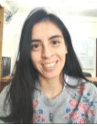
\includegraphics[width=1in,height=1.25in,clip,keepaspectratio]{./figures/mg.png}}]{María Guadalupe Gramajo}
 Recibió el título de Ingeniero en Sistemas de Información en la Universidad Tecnológica Nacional, Facultad Regional Tucumán en el año 2015. Actualmente, se desempeña como becario doctoral en el Centro de Investigación y Desarrollo de Ingeniería en Sistemas de Información, Santa Fe, Argentina. Es miembro activo y voluntaria IEEE, Sección Argentina. Sus principales áreas de investigación incluyen Ingeniería de Requerimientos, Aprendizaje Automático y Big Data.
\end{IEEEbiography}
%\newpage
% if you will not have a photo at all:
\begin{IEEEbiography}[{\includegraphics[width=1in,height=1.25in,clip,keepaspectratio]{./figures/LB.jpg}}]{Luciana C. Ballejos}
  Recibió el título de Doctor con mención Ingeniería en Sistemas de Información en la Universidad Tecnológica Nacional, Facultad Regional Santa Fe en el año 2009. En la actualidad, se desempeña como investigador docente en el Centro de Investigación y Desarrollo de Ingeniería en Sistemas de Información, Santa Fe, Argentina. Sus áreas de investigación incluyen Ingeniería del Software, Aprendizaje Automático y Cloud Computing.
\end{IEEEbiography}

% insert where needed to balance the two columns on the last page with
% biographies

\vfill

\newpage

\begin{IEEEbiography}[{\includegraphics[width=1in,height=1.25in,clip,keepaspectratio]{./figures/MA.png}}]{Mariel A. Ale}
Recibió el título de Doctor con mención Ingeniería en Sistemas de Información en la Universidad Tecnológica Nacional, Facultad Regional Santa Fe, en el año 2009. Actualmente, se desempeña como investigador docente en el Centro de Investigación y Desarrollo en Ingeniería en Sistemas de Información, Santa Fe, Argentina. Sus principales áreas de investigación incluyen, Aprendizaje Automático, Interoperabilidad Semántica y Entornos e-learning.
\end{IEEEbiography}

% You can push biographies down or up by placing
% a \vfill before or after them. The appropriate
% use of \vfill depends on what kind of text is
% on the last page and whether or not the columns
% are being equalized.

%\vfill

% Can be used to pull up biographies so that the bottom of the last one
% is flush with the other column.
%\enlargethispage{-5in}



% that's all folks
\end{document}


